\documentclass[12pt,a4paper,oneside]{easysparc}

\usepackage{amsmath,amsfonts,mathdots,amssymb}
\usepackage{graphicx}
\usepackage{subcaption}
\usepackage{lipsum}
\usepackage{indentfirst}
\usepackage{makecell}
\usepackage{booktabs}
\usepackage{algpseudocode, algorithm}
\usepackage{hyperref}
\usepackage{pdfpages}

\DeclareMathOperator*{\argmin}{arg\,min}

\floatname{algorithm}{Algoritmo}

% % % % % % % % % % % % % % % % % % % % % % % % % % %
% Pacotes adicionados % % % % % % % % % % % % % % % %
% % % % % % % % % % % % % % % % % % % % % % % % % % %

%% % % % % % %
\onehalfspacing{}
\begin{document}
\sloppy
% % % % % % % % % % % % % % % % % % % % % % % % % % %
\author{
    Hugo Tallys Martins Oliveira
}
\docTitle{
    Resolução de Redundância aplicada a um manipulador robótico com cinco graus de liberdade
}

\docType{1}	%% TCC=1; Qualificação Mestrado=2; Dissertação=3; Qualificação Doutorado=4; Tese=5;

% % % % % % % % % % % % % % % % % % % % % % % % % % % % % %
% % % % % % % % % % % % % % % % % % % % % % % % % % % % % %

\orientador{Glauber Rodrigues Leite} %% Nome 
\tituloOrientador{Prof.\ Dr.} %% Titulo, Instituição

\coorientador{} %% Nome
\tituloCoorientador{} %% Título, Instituição

\memberA{Ícaro Bezerra Queiroz de Araújo} %% Nome
\filiationA{Prof.\ Dr., UFAL} %% Titulo, Instituição

\memberB{Arthur da Costa Vangasse} %% Nome
\filiationB{Msc., UFMG} %% Titulo, Instituição

\memberC{} %% Nome
\filiationC{} %% Titulo, Instituição

\memberD{} %% Nome
\filiationD{} %% Titulo, Instituição

\memberE{} %% Nome
\filiationE{} %% Titulo, Instituição

% % % % % % % % % % % % % % % % % % % % % % % % % % % % % %
% % % % % % % % % % % % % % % % % % % % % % % % % % % % % %

\setDate{26}
\setMonth{Julho}
\setYear{2024}
\setLocation{Maceió, Alagoas}

% % % % % % % % % % % % % % % % % % % % % % % % % % % % % %
% % % % % % % % % % % % % % % % % % % % % % % % % % % % % %	% % % % % % % % % % % % % % %
% % % % % % % % % % % % % % % % % % % % % % % % % % %
\capa{}
\folhaDeRosto{}
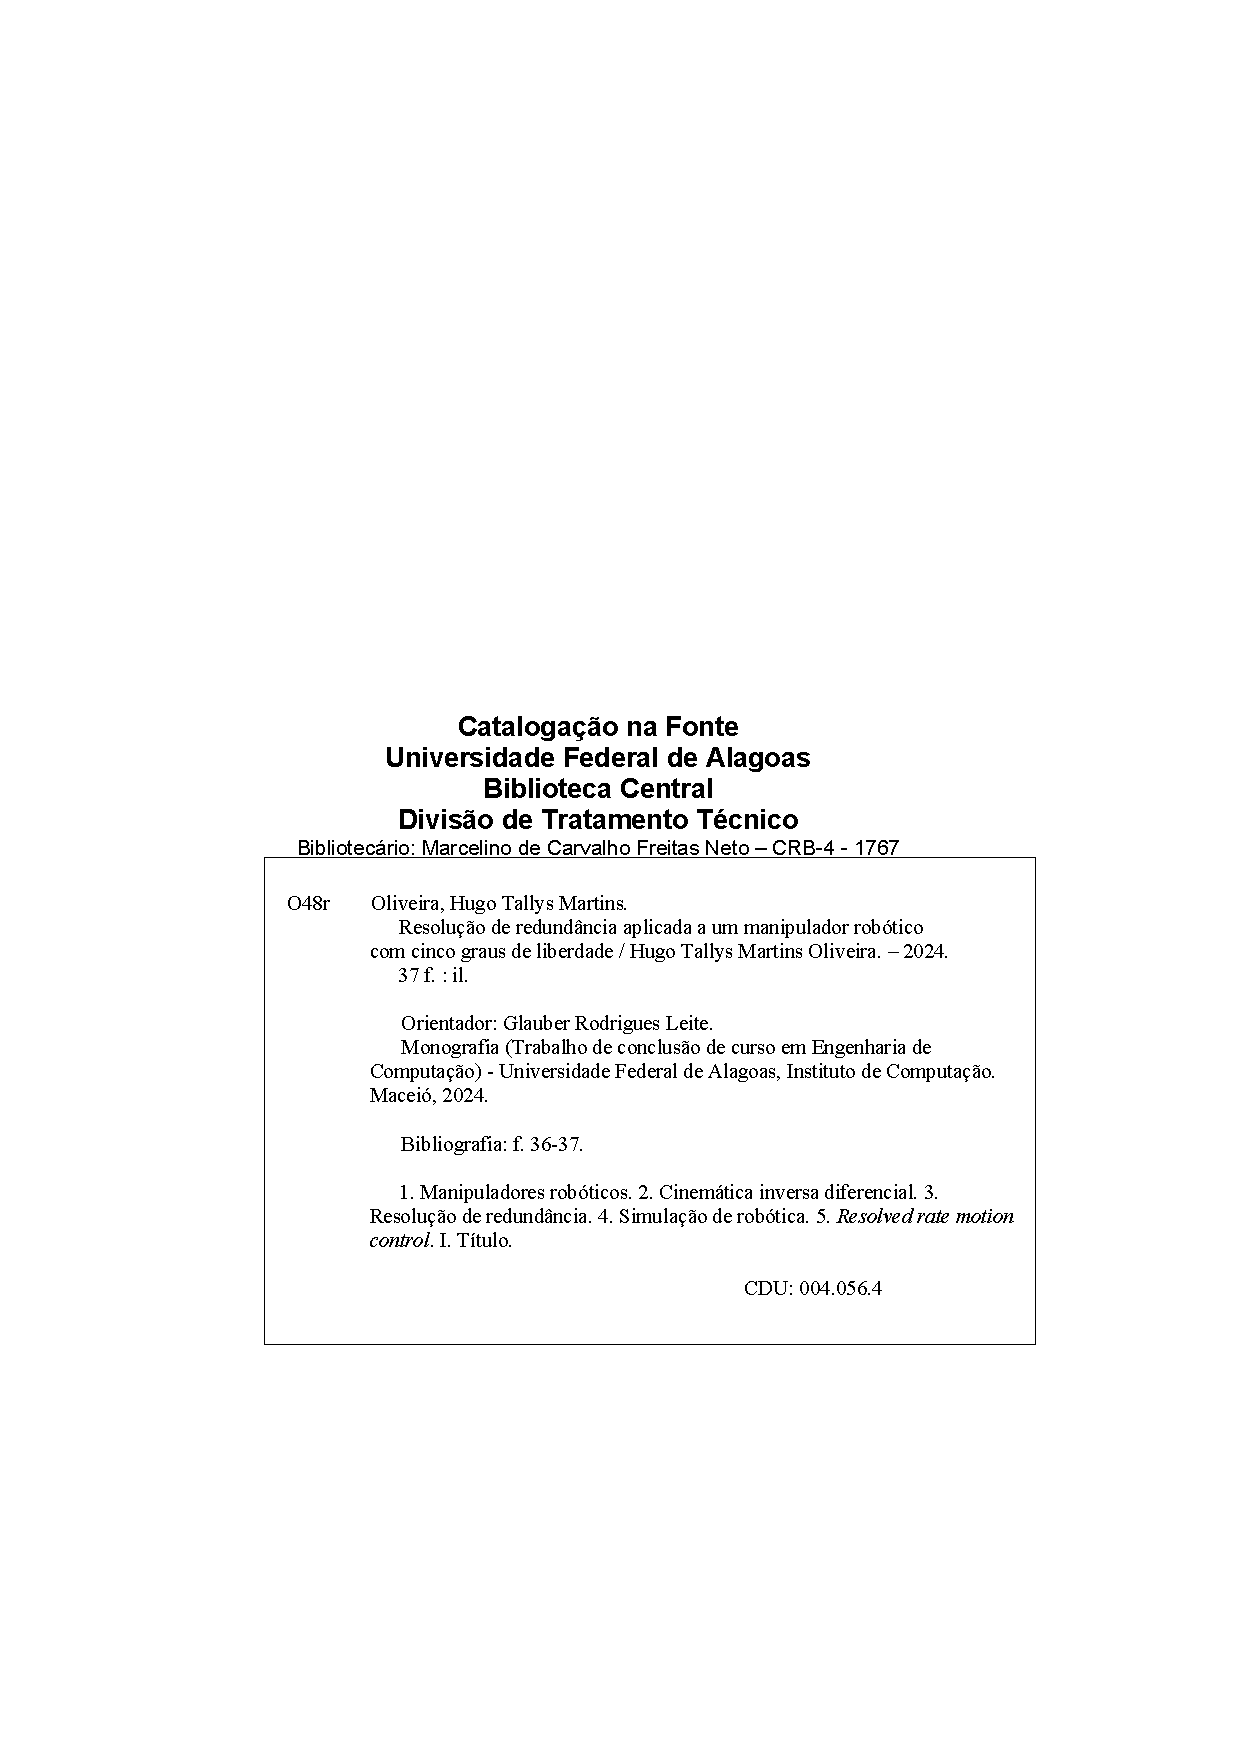
\includepdf{./ficha-catalografica.pdf}
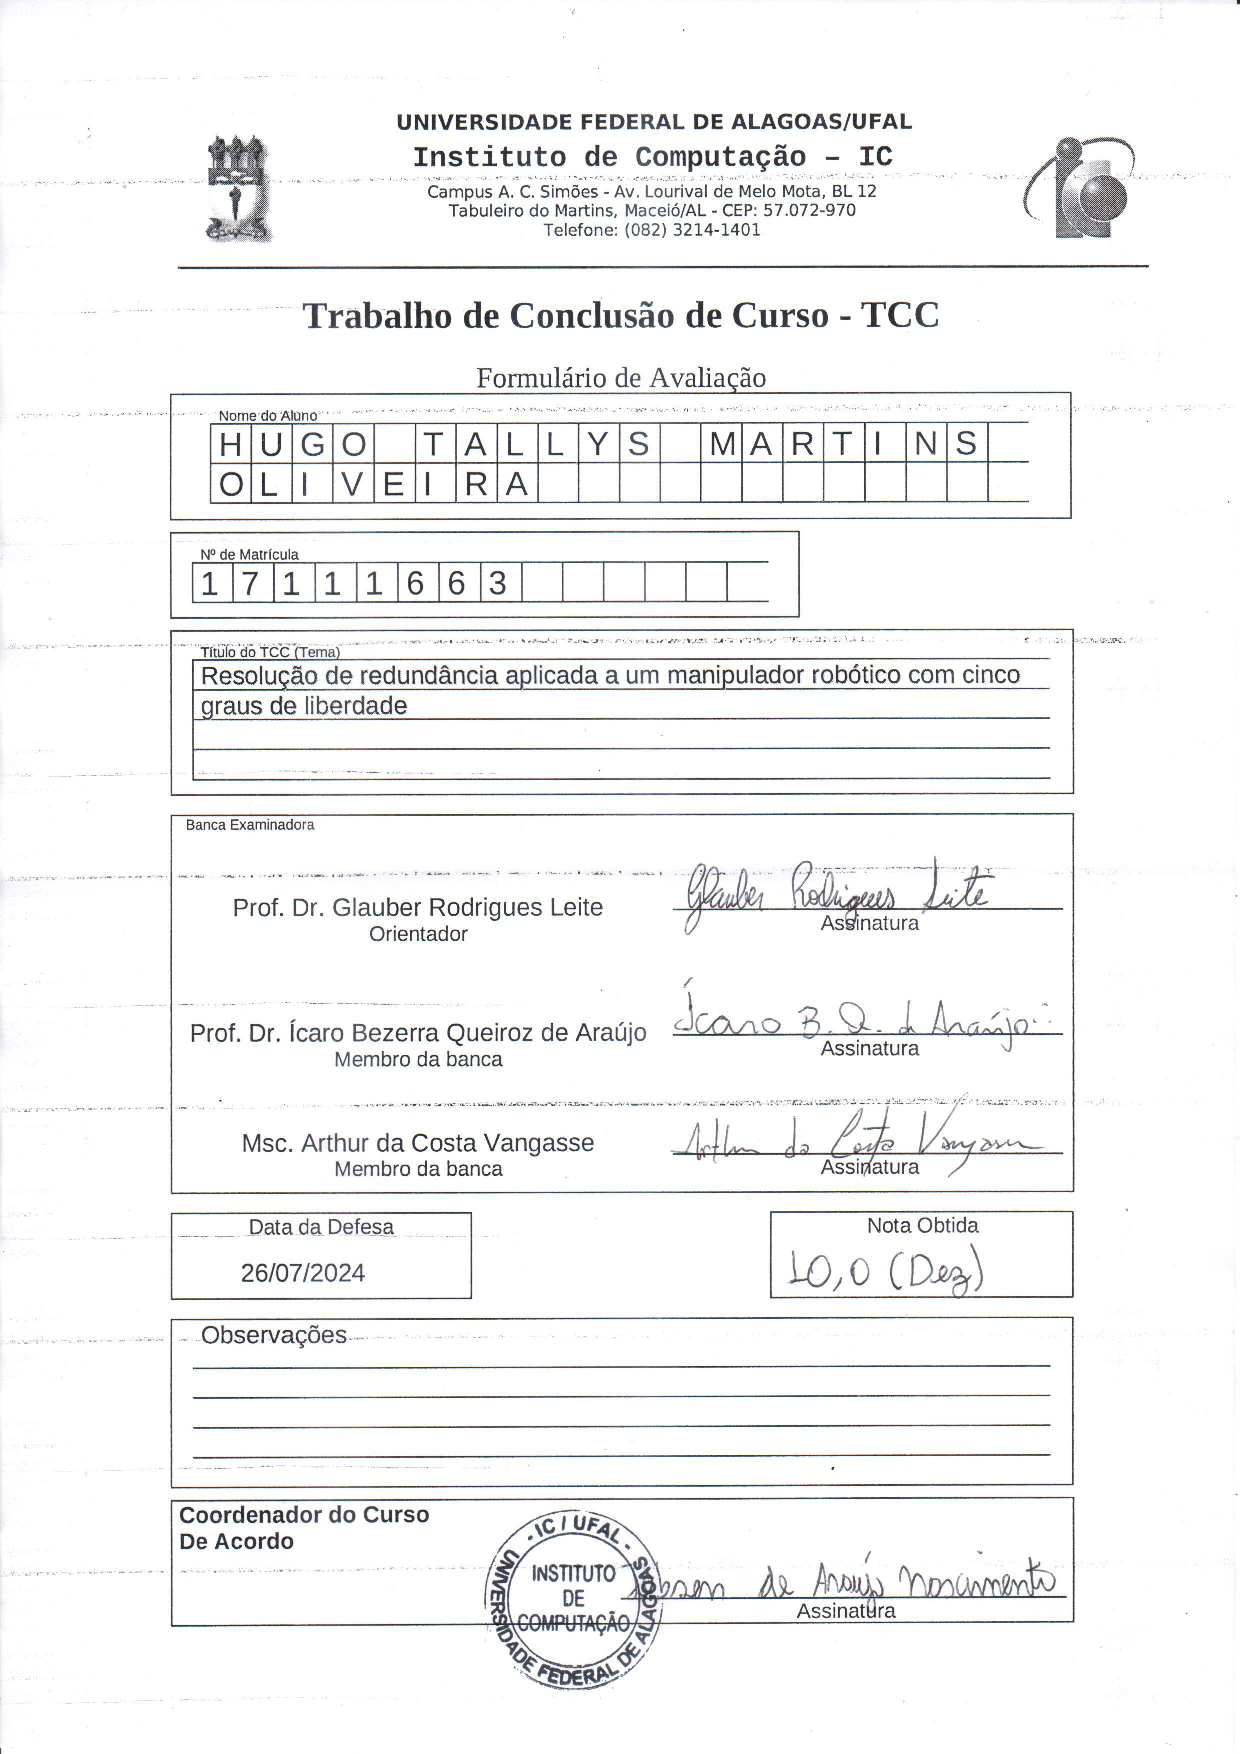
\includepdf{./ata-assinada.pdf}
%\folhaDeAprovacao{}

% % % % % % % % % % % % % % % % % % % % % % % % % % %
% Opcionais % % % % % % % % % % % % % % % % % % % % %
% % % % % % % % % % % % % % % % % % % % % % % % % % %
\dedicatoria{} % opcional
\agradecimentos{} % opcional
\epigrafe{} % opcional

% % % % % % % % % % % % % % % % % % % % % % % % % % %
% Obrigatórios  % % % % % % % % % % % % % % % % % % % 
% % % % % % % % % % % % % % % % % % % % % % % % % % %
\resumo{}
\abstract{}
% % % % % % % % % % % % % % % % % % % % % % % % % % %
% % % % % % % % % % % % % % % % % % % % % % % % % % %
\listoffigures
\cleardoublepage{}
% % % % % % % % % % % % % % % % %
\listoftables
\cleardoublepage{}
\simbolos{}
\cleardoublepage{}
\abreviaturas{}
\cleardoublepage{}
% % % % % % % % % % % % % % % % % % % % % % % % % % %
% % % % % % % % % % % % % % % % % % % % % % % % % % %
\renewcommand{\contentsname}{Sumário}
\tableofcontents
\cleardoublepage{}
% % % % % % % % % % % % % % % % % % % % % % % % % % %
% % % % % % % % % % % % % % % % % % % % % % % % % % %
\pagenumbering{arabic}

\pagestyle{myheadings}
\renewcommand{\chaptermark}[1]{\markboth{#1}{}}
\renewcommand{\sectionmark}[1]{\markright{#1}}

% % % % % % % % % % % % % % % % % % % % % % % % % % %
% Incluir capítulos aqui  % % % % % % % % % % % % % %
% % % % % % % % % % % % % % % % % % % % % % % % % % %
\chapter{Introdução}\label{cap:introduction}

A redundância cinemática na robótica refere-se ao uso de graus de liberdade, em inglês \emph{degrees of freedom} (DoF) adicionais além do mínimo necessário para executar uma
tarefa específica. Em robôs industriais e manipuladores, singularidades cinemáticas ocorrem quando a configuração do robô resulta na perda
de um ou mais DoFs, reduzindo sua capacidade de movimento. De maneira mais precisa, isso significa que há alguma direção (ou subespaço) 
no espaço cartesiano ao longo da qual é impossível mover o efetuador final, independentemente das velocidades empenhadas nas 
juntas~\cite{craig2004}. 

A importância da redundância está na capacidade de fornecer caminhos alternativos para o planejamento de movimentos,
permitindo que o robô manobre ao redor de configurações singulares, mantendo a eficiência operacional e a segurança. Essa flexibilidade 
assegura que o robô continue a executar suas tarefas mesmo próximo a pontos singulares, comuns em tarefas complexas. Além disso, a resolução
de redundância possibilita a otimização de outros critérios de desempenho, como minimizar o consumo de energia, reduzir o desgaste, melhorar 
a precisão e aumentar a capacidade de evasão de obstáculos.

Recentemente,~\cite{li2023pseudo} propuseram um novo esquema de \emph{Obstacle avoidance} (OA) para manipuladores redundantes 
baseado em na pseudo-inversa da matriz jacobiana no nível das acelerações das juntas, demonstrando a viabilidade do método através de simulações 
com o manipulador robótico PA10 o qual possui \(7\) DoFs. Por outro lado,~\cite{kuri2023som}
abordaram uma técnica de controle inteligente para um manipulador robótico espacial com 5 DoFs para executar
trajetórias tridimensionais desejadas (linha, circular e elíptica) enquanto resolve a redundância 
(evitação dos limites das juntas) mostrando que a depender da tarefa, mesmo para manipuladores com um número menor de DoFs, 
a redundância pode ser explorada para melhorar o desempenho do robô.

O trabalho de \cite{ancona2017} validou técnicas de resolução de redundância em diversos cenários, destacando a importância da escolha do critério de desempenho
para direcionar o comportamento do manipulador. A metodologia proposta, baseada em um procedimento de cinemática inversa e um controlador orientado a objetos,
mostrou-se eficaz e versátil tanto em simulações quanto na prática real. Além disso, o trabalho explorou a manipulação móvel redundante para operações hábeis 
e interação segura entre humanos e robôs em ambientes industriais, com uma contribuição importante na arquitetura de controle de software proposta, que é escalável,
portátil, integrável com tecnologias heterogêneas e pronta para uso em ambientes de produção.

Por fim, \cite{hammond2011} propôs um método heurístico para configurar manipuladores robóticos com redundância cinemática, visando aumentar a precisão 
dos movimentos em tarefas específicas, utilizando o índice de resolução de movimento efetivo (EMR). Os resultados mostram que o índice EMR pode ser 
usado tanto como uma métrica de aptidão em otimização de design quanto como um objetivo na resolução de redundância,  destacando o potencial dessas
abordagens em aplicações de micromanipulação e montagem de precisão,  melhorando significativamente a resolução de movimento em trajetórias específicas 
sem a necessidade de componentes de alta precisão e custo elevado.

\section{Motivação}\label{sec:motivation}

A abordagem tradicional no projeto de manipuladores teve como foco principal a minimização de custos e manutenção,
utilizando o número mínimo de juntas necessárias para uma executar uma determinada tarefa levando, por exemplo, ao
desenvolvimento dos robôs \emph{Selective Compliance Assembly Robot Arm} (SCARA) para operações de \emph{pick-and-place}~\cite{siciliano_springer_2008}.
No entanto, essa abordagem  minimalista apresenta uma série de limitações em aplicações do mundo real, onde fatores como
limites de juntas, singularidades e obstáculos no espaço de trabalho estão presentes. Ao ter mais DoFs
do que o estritamente necessário, os manipuladores redundantes podem alcançar maior destreza e versatilidade, tornando-os
mais adequados para ambientes complexos e dinamicamente mutáveis.

Para além das restrições cinemáticas, a redundância permite a otimização de métricas de desempenho, como a minimização do torque ou do consumo de energia, melhorando a
eficiência geral do sistema. Vale ressaltar que projetar manipuladores com juntas adicionais e garantir sua confiabilidade operacional é um
processo complexo e custoso. Esquemas eficazes de resolução de redundância são críticos para o sucesso do planejamento e controle de movimentos,
especialmente em ambientes dinâmicos. Apesar desses desafios, os benefícios da redundância cinemática em aumentar a destreza, versatilidade e eficiência
fazem dela uma abordagem interessante em sistemas robóticos avançados.

\section{Objetivos}\label{sec:objectives}

\subsection{Objetivos Gerais}

Estudar e implementar a modelagem de cinemática inversa diferencial em manipuladores seriais redundantes, possibilitando a execução de
trajetórias no espaço de trabalho que levam em conta não só as restrições cinemáticas do movimento mas também critérios
de desempenho do manipulador.

\subsection{Objetivos Específicos}
\begin{itemize}
	\item Estudar a modelagem de cadeias cinemáticas em manipuladores robóticos seriais
	\item Investigar o uso da cinemática direta e inversa diferenciais para execução de trajetórias cartesianas
	\item Implementar a lei de controle utilizando a cinemática direta diferencial e esquemas de resolução de redundância utilizando a pseudo inversa da matriz jacobiana
	\item Propor um ambiente virtual para execução de simulações utilizando o modelo de um manipulador robótico com 5 graus de liberdade
	\item Analisar o desempenho do esquema de controle em diferentes cenários de execução de trajetórias e critérios de desempenho.
\end{itemize}

\section{Estrutura do texto}\label{sec:structure}

Este trabalho está estruturado de modo a introduzir os conceitos já difundidos da cinemática diferencial em manipuladores redundantes,
bem como apresentar uma abordagem prática para resolução de redundância de um manipulador planar simples, com cinco graus de liberdade.
No capítulo 2, é apresentada a fundamentação teórica, abordando conceitos essenciais como a representação de poses no
espaço, transformações homogêneas, cinemática direta, cinemática diferencial, e a resolução de redundância.
O capítulo 3 descreve a implementação prática, detalhando a simulação de manipuladores robóticos, a arquitetura de comunicação proposta
e o algoritmo \emph{Resolved Rate Motion Control}. No capítulo 4, são apresentados os resultados experimentais divididos em dois cenários
distintos, seguidos pela conclusão no capítulo 5, onde são discutidos os principais pontos abordados e sugestões para trabalhos futuros.

\cleardoublepage{}
% % % % % % % % % % % % % % % % % % % % % % % % % % %
\chapter{Fundamentação teórica}\label{cap:background}

\section{Poses no espaço}

O estudo da cinemática na robótica envolve principalmente o estabelecimento de
sistemas de coordenadas (em inglês, \emph{frames}) para representar posições e
orientações de corpos rígidos, além da caracterização das transformações entre
esses frames. Nesta seção, definiremos uma forma precisa para representar
translações e rotações no espaço por meio de matrizes e vetores. Em seguida,
apresentaremos as transformações homogêneas, que combinam as operações de
rotação e translação em uma única multiplicação matricial, proporcionando uma
maneira concisa de estabelecer a relação entre dois frames distintos.

\subsection{Representado posições e orientações no espaço}

Um sistema de coordenadas ou \emph{frame} é definido por um ponto e um conjunto
de vetores ortonormais que formam uma base no espaço considerado (dois vetores
no plano e três vetores no espaço tridimensional). No contexto da robótica é
muito comum a especificação de uma tarefa com base em coordenadas cartesianas
relativas a algum frame de referência como ilustrado na
figura~\ref{fig:frames}. Podemos tomar o \emph{frame} \(o_0 x_0 y_0 z_0\) como
referência e expressar qualquer ponto \(P\) do espaço através de um vetor com
origem em \(o_0\) e extremidade em \(P\) de modo que escreveríamos:

\begin{equation}
    p^0 = v_0^0 = \begin{bmatrix}
        1 \\
        1 \\
        1
    \end{bmatrix}
\end{equation}

onde o expoente \(0\) indica que o vetor é expresso com coordenadas referentes
ao \emph{frame} \(o_0 x_0 y_0 z_0\). Contudo, ainda observando a
figura~\ref{fig:frames}, podemos expressar o mesmo ponto \(P\) com coordenadas
referentes ao \emph{frame} \(o_1 x_1 y_1 z_1\) através do vetor \(v_1^1\) de
modo que, teríamos por exemplo:

\begin{equation}
    p^1 = v_1^1 = \begin{bmatrix}
        2    \\
        -1.5 \\
        3
    \end{bmatrix}
\end{equation}

Além disso, poderíamos também calcular \(v_1^0\) e \(v_0^1\) de modo que as
coordenadas do vetor dependem do sistema de referência utilizado.

\begin{figure}
    \centering
    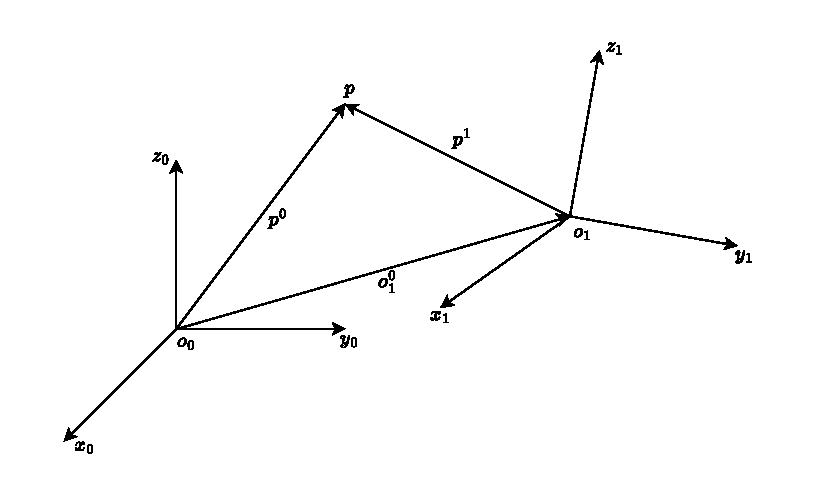
\includegraphics[width=0.8\linewidth]{Images/frames.pdf} % Adjust the width as needed
    \caption{Dois sistemas de coordenadas, um ponto P e vetores que o representam.}\label{fig:frames}
\end{figure}

Para estabelecer a relação completa entre os dois \emph{frames} precisamos
também considerar a orientação de um com relação ao outro. Podemos expressar
relação de orientação entre os \emph{frames} \(\{0\}\) e \(\{1\}\) utilizando a
matriz de mudança de base \(R_1^0\) dada por:

\begin{equation}
    R_1^0 = \begin{bmatrix}
        x_1 \cdot x_0 & y_1 \cdot x_0 & z_1 \cdot x_0 \\
        x_1 \cdot y_0 & y_1 \cdot y_0 & z_1 \cdot y_0 \\
        x_1 \cdot z_0 & y_1 \cdot z_0 & z_1 \cdot z_0
    \end{bmatrix}
\end{equation}

onde \((\cdot)\) denota o produto escalar entre dois vetores.

A matriz \(R_1^0\) faz parte de um conjunto de matrizes denominado grupo
especial ortogonal de ordem 3 (\(SO(3)\)) que possui algumas propriedades
interessantes dentre elas a facilidade de se calcular sua inversa:

\begin{equation}
    {(R_1^0)}^{-1} = {(R_1^0)}^{\top} = R_0^1
\end{equation}

Se a relação entre os \emph{frames} é composta apenas por uma rotação de
\(\theta\) radianos em torno de cada eixo ordenado, podemos calcular as
seguintes matrizes de transformação elementares:

\begin{equation}
    R_x(\theta) = \begin{bmatrix}
        1 & 0            & 0             \\
        0 & \cos(\theta) & -\sin(\theta) \\
        0 & \sin(\theta) & \cos(\theta)
    \end{bmatrix}
\end{equation}

\begin{equation}
    R_y(\theta) = \begin{bmatrix}
        \cos(\theta)  & 0 & \sin(\theta) \\
        0             & 1 & 0            \\
        -\sin(\theta) & 0 & \cos(\theta)
    \end{bmatrix}
\end{equation}

\begin{equation}
    R_z(\theta) = \begin{bmatrix}
        \cos(\theta) & -\sin(\theta) & 0 \\
        \sin(\theta) & \cos(\theta)  & 0 \\
        0            & 0             & 1
    \end{bmatrix}
\end{equation}

\subsection{Transformações homogêneas}

Um deslocamento rígido no espaço pode ser representado por uma translação pura
seguida de uma rotação pura. De maneira mais precisa, podemos defini-lo como um
par ordenado \((R, d)\) onde \(R \in SO(3)\) e \(d \in \mathbb{R}^3\). O grupo
de todas as transformações rígidas no espaço tridimensional é denominado grupo
especial euclidiano de ordem 3 (\(SE(3)\)) onde vemos claramente que \(SE(3) =
\mathbb{R}^3 \times SO(3)\).

Seja \(R_1^0\) a matriz de rotação que especifica a orientação do sistema de
coordenadas \(\{1\}\) com relação ao sistema de coordenadas \(\{0\}\) e
\(o_1^0\) o vetor de deslocamento une suas origens. Como visto ne seção
anterior, se \(P\) é um ponto fixado ao sistema de coordenadas \(\{1\}\) com
coordenadas locais dadas por \(p^1\) então, podemos expressar as coordenadas de
\(P\) com relação ao sistema de coordenadas \(\{0\}\) usando o seguinte
deslocamento rígido:

\begin{equation}\label{eq:rigid-motion}
    p^0 = R_1^0 p^1 + o_1^0
\end{equation}

A equação (\ref{eq:rigid-motion}) pode ser reescrita de maneira mais compacta
utilizando-se a seguinte formulação matricial:

\begin{equation}
    \begin{bmatrix}
        p^0 \\
        1
    \end{bmatrix} = \begin{bmatrix}
        R_1^0 & o_1^0 \\
        0     & 1
    \end{bmatrix} \begin{bmatrix}
        p^1 \\
        1
    \end{bmatrix} \ \ , R_1^0 \in SO(3) \ \ , o_1^0 \in \mathbb{R}^3
\end{equation}

onde vemos que os elementos de \(SE(3)\) são matrizes de dimensão \(4 \times
4\) e os vetores \(p^i\) são representados em \emph{coordenadas homogêneas }com
uma dimensão extra. A matriz \(T_1^0\) é denominada matriz de
\emph{transformação homogênea} e utilizando o fato de que \(R_1^0\) é uma
matriz ortogonal, podemos facilmente calcular sua inversa:

\begin{equation}
    {(T_1^0)}^{-1} = \begin{bmatrix}
        R_1^0 & o_1^0 \\
        0     & 1
    \end{bmatrix}^{-1} = \begin{bmatrix}
        {(R_1^0)}^{\top} & -{(R_1^0)}^{\top} o_1^0 \\
        0                & 1
    \end{bmatrix}
\end{equation}

\section{Cinemática Direta}

O problema da cinemática em manipuladores consiste em descrever o movimento do
manipulador sem considerar as forças e torques atuantes sob o mesmo
tratando-se, portanto, de uma descrição puramente geométrica. Neste contexto,
uma pergunta natural que surge é como podemos determinar a posição e orientação
do efetuador final na cadeia cinemática dado um conjunto arbitrário de ângulos
articulados. Este problema é conhecido na robótica como a cinemática direta de
um manipulador e pode ser facilmente resolvido se associarmos a cada corpo
rígido da cadeia um sistema de coordenadas (\emph{frame}), expressando também
as relações entre esses \emph{frames} como transformações homogêneas. A pose do
efetuador final fica determinada através de uma série de multiplicações
matriciais. A colocação de \emph{frames} pode ser feita de maneira sistemática
através da utilização da convenção de Denavit-Hartenberg a qual fornece uma
abordagem concisa para representar a estrutura geométrica do manipulador.

\subsection{Cadeias cinemáticas}

Na robótica, uma cadeia cinemática pode ser definida como uma série de corpos
rígidos, também denominados \emph{elos}, conectados por \emph{juntas} que
permitem um movimento relativo das diferentes partes móveis de um manipulador.
Cadeias cinemáticas formam a base do estudo de manipuladores robóticos e
geralmente são representadas através de um grafo onde seus nós constituem os
elos e as arestas as juntas.

Dependendo da topologia desse grafo, podemos classificar uma cadeia cinemática
de diferentes formas. Numa cadeia serial aberta seu grafo consiste numa árvore
onde cada nó possui apenas um único filho e o nó terminal da árvore usualmente
representa o efetuador final (onde uma pinça ou garra robótica ficaria
acoplada, por exemplo). Outros casos incluem grafos com ramificações (existe
mais de um nó terminal) onde denominamos de cadeia paralela ou quando há a
presença de ciclos onde temos uma cadeia fechada. Neste trabalho, iremos nos
limitar à análise de cadeias abertas, as mais comuns no âmbito de manipuladores
robóticos utilizados em aplicações industriais.

Os tipos de juntas presentes no cadeia também são importantes na definição do
alcance e natureza do movimento do manipulador. As mais simples são as juntas
prismáticas e de revolução, cada uma introduzindo um único grau de liberdade ao
sistema. Juntas prismáticas permitem o movimento translacional ao longo de uma
única direção enquanto que juntas de revolução possibilitam um movimento
rotacional ao redor de um eixo específico.

Ademais das juntas básicas, tipos mais complexos incluem juntas esféricas, que
introduzem dois graus de liberdade (rotação ao redor de dois eixos
perpendiculares) e punhos esféricos, compostos por três juntas revolutas
dispostas ortogonalmente, introduzindo três graus de liberdade ao sistema. Vale
ressaltar que independente da complexidade da junta, a maior parte pode ser
reduzida a uma combinação dos dois tipos mais simples tornando suficiente a
descrição de cadeias cinemáticas por meio de uma combinação de juntas
prismáticas ou de revolução.

Um manipulador robótico com $n$ juntas terá $n + 1$ elos, uma vez que cada
junta conecta exatamente dois elos. Iremos enumerar as juntas de $1$ até $n$ e
elos de $0$ a $n$ sendo que o elo de número $0$ representará a base do
manipulador e elo $n$ seu efetuador final. De acordo com essa convenção a junta
$i$ conecta os elos $i - 1$ ao $i$ e tem sua posição fixa com respeito ao elo
anterior. Quando a junta $i$ é atuada, o elo $i$ se movimenta de modo que a
base permanece fixa independente de qual junta é movimentada.

Iremos associar à $i$-ésima junta uma variável $q_i$ representando no caso de
uma junta de revolução o ângulo de rotação e no caso de uma junta prismática o
deslocamento linear:

\begin{equation}
    q_i =
    \begin{cases}
        \theta_i & \text{se a junta $i$ é de revolução} \\
        d_i      & \text{se a junta $i$ é prismática}   \\
    \end{cases}
\end{equation}

A análise cinemática é feita anexando ao elo $i$ da cadeia o sistema de
coordenadas $o_i x_i y_i z_i$. O \emph{frame} $o_0 x_0 y_0 z_0$ associado à
base do manipulador é denominado \emph{frame} da base, inercial ou do mundo. Se
$A_i(q_i)$ é a matriz de transformação homogênea que fornece a posição e
orientação de $o_i x_i y_i z_i$ com relação a $o_{i-1} x_{i-1} y_{i-1} z_{i-1}$
então podemos dizer que a mesma é função unicamente da variável $q_i$ de modo
que:

\begin{equation}
    A(q_i) = A_i = \begin{bmatrix}
        R^{i-1}_i & o^{i-1}_i \\
        0         & 1
    \end{bmatrix}
\end{equation}

Dessa forma, para $i < j$, a matriz $T_j^i$ dada por:

\begin{equation}
    T_j^i = A_{i+1} \cdots A_j = \begin{bmatrix}
        R^i_j & o^i_j \\
        0     & 1
    \end{bmatrix}
\end{equation}

expressa a orientação $R^i_j$ e posição $o^i_j$ de $o_j x_j y_j z_j$ com
relação a $o_i x_i y_i z_i$. Vale ressaltar que a matriz $R^i_j$ é calculada
através da multiplicação matricial:

\begin{equation}
    R^i_j = R^i_{i+1} \cdots R^{j-1}_j
\end{equation}

e o vetor de posição utilizando-se a seguinte equação recursiva:

\begin{equation}
    o^i_j = o^i_{j-1} + R^i_{j-1}o^{j-1}_j
\end{equation}

O problema da cinemática direta pode ser então formulado como o simples cálculo
da matriz $T^0_n$ que expressa a pose do efetuador final com relação ao
\emph{frame} da base:

\begin{equation}\label{eq:fkine}
    T^0_n = A_1 A_2 \cdots A_n = \begin{bmatrix}
        R^0_n & o^0_n \\
        0     & 1
    \end{bmatrix}
\end{equation}

Tendo em vista a infinidade de possibilidades de se anexar os \emph{frames} em
cade elo, para poder calcular as matrizes $A_i$ de forma mais precisa, vamos
estabelecer uma convenção utilizando para isso os parâmetros introduzidos por
Denavit e Hartenberg.

\subsection{Convenção de Denavit-Hartenberg}

A fixação de frames em cada elo pode ser feita de maneira arbitrária para se
obter as matrizes de transformação $A_i$, permitindo assim o cálculo da
cinemática direta. Contudo, o processo de determinação das mesmas matrizes para
um manipulador com $n$ elos começa a ser tornar cada vez mais complexo a medida
que $n$ cresce. A a convenção de Denavit-Hartenberg consiste numa abordagem
sistemática para a obtenção das matrizes $A_i$ de modo a representar a relação
entre frames consecutivos da forma mais concisa o possível além de propiciar
uma padronização de como pesquisadores descrevem a estrutura cinemática de um
manipulador robótico.

De maneira geral, para especificar a matriz de transformação homogênea seriam
necessários 6 parâmetros: três deslocamentos para a componente de translação e
três ângulos para a rotação. Na convenção de Denavit-Hartenberg, a matriz de
transformação $A_i$ associada ao $i$-ésimo elo é descrita através de apenas 4
parâmetros. Isso é obtido através da introdução de duas restrições na colocação
dos frames em cada elo:

\begin{itemize}
    \item (\textbf{DH1}) $x_i$ intersecta o eixo $z_{i-1}$
    \item (\textbf{DH2}) $x_i$ é perpendicular o eixo $z_{i-1}$
\end{itemize}

\begin{figure}
    \centering
    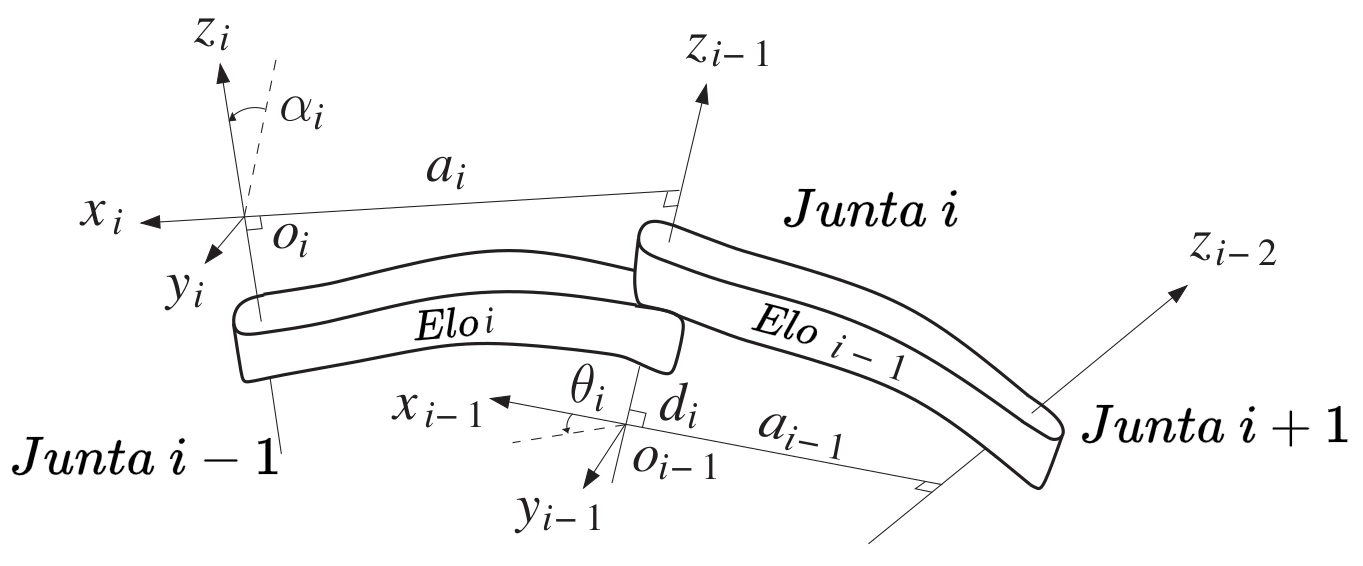
\includegraphics[width=0.8\linewidth]{Images/dh-assignment.png}
    \caption{Atribuição de \emph{frames} de acordo com a convenção de Denavit-Hartenberg. Adaptado de~\cite{spong_robot_2020}.}\label{fig:dh-assignment}
\end{figure}

O cálculo da matriz $A_i$ fica condicionado à determinação dos parâmetros:
$\theta_i$ (joint angle), $d_i$ (link offset), $a_i$ (link length) e $\alpha_i$
(link twist). Como $A_i$ é função da única variável da junta, três parâmetros
são sempre fixos, dependendo apenas da geometria existente entre os frames,
enquanto o quarto parâmetro é livre: $\theta_i$, no caso de uma junta de
revolução e $d_i$, no caso de uma junta prismática. Em posse dos parâmetros
obtidos para cada par de elos consecutivos, o cálculo da matriz $A_i$ é obtido
através da relação:

\begin{align}
    A_i & = Rot_z(\theta_i) \cdot Trans_z(d_i) \cdot Trans_x(a_i) \cdot Rot_x(\alpha_i)             \\
    A_i & = \begin{bmatrix}
                c_{\theta_i} & -s_{\theta_i} & 0 & 0 \\
                s_{\theta_i} & c_{\theta_i}  & 0 & 0 \\
                0            & 0             & 1 & 0 \\
                0            & 0             & 0 & 1
            \end{bmatrix} \begin{bmatrix}
                              1 & 0 & 0 & 0   \\
                              0 & 1 & 0 & 0   \\
                              0 & 0 & 1 & d_i \\
                              0 & 0 & 0 & 1
                          \end{bmatrix} \notag                                                    \\
        & \phantom{=} \times \ \ \begin{bmatrix}
                                     1 & 0 & 0 & a_i \\
                                     0 & 1 & 0 & 0   \\
                                     0 & 0 & 1 & 0   \\
                                     0 & 0 & 0 & 1
                                 \end{bmatrix} \begin{bmatrix}
                                                   1 & 0            & 0             & 0 \\
                                                   0 & c_{\alpha_i} & -s_{\alpha_i} & 0 \\
                                                   0 & s_{\alpha_i} & c_{\alpha_i}  & 0 \\
                                                   0 & 0            & 0             & 1
                                               \end{bmatrix} \notag                 \\
    A_i & = \begin{bmatrix}
                c_{\theta_i} & -s_{\theta_i}c_{\alpha_i} & s_{\theta_i}s_{\alpha_i}  & a_i c_{\theta_i} \\
                s_{\theta_i} & c_{\theta_i}c_{\alpha_i}  & -c_{\theta_i}s_{\alpha_i} & a_i s_{\theta_i} \\
                0            & s_{\alpha_i}              & c_{\alpha_i}              & d_i              \\
                0            & 0                         & 0                         & 1
            \end{bmatrix} \label{eq:dh-matrix}
\end{align}

onde $c_{\cdot}$ e $s_{\cdot}$ denotam $\cos(\cdot)$ e $\sin(\cdot)$,
respectivamente. A tabela~\ref{tab:dh-parameters} descreve de maneira detalhada
a definição de cada parâmetro de Denavit-Hartenberg.

\begin{table}[htbp]
    \centering
    \begin{tabular}{c c}
        \toprule
        \textbf{Parâmetro} & \textbf{Definição}                                                                                             \\
        \midrule
        $\theta_i$         & \makecell[l]{O ângulo entre os eixos $\mathbf{x}_{i-1}$ e $\mathbf{x}_i$ em torno do eixo $\mathbf{z}_{i-1}$}  \\
        \midrule
        $d_i$              & \makecell[l]{A distância da origem do sistema de coordenadas $\{i-1\}$                                         \\ até o eixo $\mathbf{x}_i$ ao longo do eixo $\mathbf{z}_{i-1}$} \\
        \midrule
        $a_i$              & \makecell[l]{A distância entre os eixos $\mathbf{z}_{i-1}$ e $\mathbf{z}_i$ ao longo do eixo $\mathbf{x}_i$;   \\ para eixos que se intersectam, é paralela a $\mathbf{z}_{i-1} \times \mathbf{z}_i$} \\
        \midrule
        $\alpha_i$         & \makecell[l]{O ângulo entre o eixo $\mathbf{z}_{i-1}$ e o eixo $\mathbf{z}_i$ em torno do eixo $\mathbf{x}_i$} \\
        \bottomrule
    \end{tabular}
    \caption{Descrição dos parâmetros Denavit-Hartenberg}\label{tab:dh-parameters}
\end{table}

\subsection{Cinemática direta de um braço planar}

Um braço planar é um tipo de manipulador serial cujo espaço de trabalho se
limita a um plano. A figura~\ref{fig:3r-planar-arm} mostra um braço planar do
tipo 3R, o qual possui três elos e três juntas de revolução acoplados em série.
A escolha da colocação do frame da base \(o_0x_0y_0z_0\) é totalmente
arbitrária e ao tomar como indicado na figura (com o eixo \(z\) apontando para
fora do papel) a fixação dos frames subsequentes na cadeia cinemática fica
restrita a convenção de Denavit-Hartenberg adotada. A tabela DH para esse
manipulador é dada por:

\begin{table}[htbp]
    \centering
    \begin{tabular}{c c c c c}
        \toprule
        \textbf{Elo} & \(\theta\)   & \(d\) & \(a\)   & \(\alpha\) \\
        \midrule
        1            & \(\theta_1\) & 0     & \(a_1\) & 0          \\
        2            & \(\theta_2\) & 0     & \(a_2\) & 0          \\
        3            & \(\theta_3\) & 0     & \(a_3\) & 0          \\
        \bottomrule
    \end{tabular}
    \caption{Parâmetros DH para o braço planar 3R da figura~\ref{fig:3r-planar-arm}.}\label{tab:dh-parameters-planar-arm}
\end{table}

Dados os valores fixos \(a_i\) que indicam o comprimento do elo \(i\), as
únicas variáveis livres no cálculo da cinemática direta são os ângulos das
juntas ($q_i = \theta_i$), desse modo, vamos denotar \(\theta_1 + \theta_2 =
\theta_{12}\), \(\cos(\theta_1 + \theta_2) = c_{12}\) e assim por diante. Para
\(i = 1, 2, 3\) as matrizes $A_i$ são calculadas com o auxílio da
equação~\ref{eq:dh-matrix}:

\begin{figure}
    \centering
    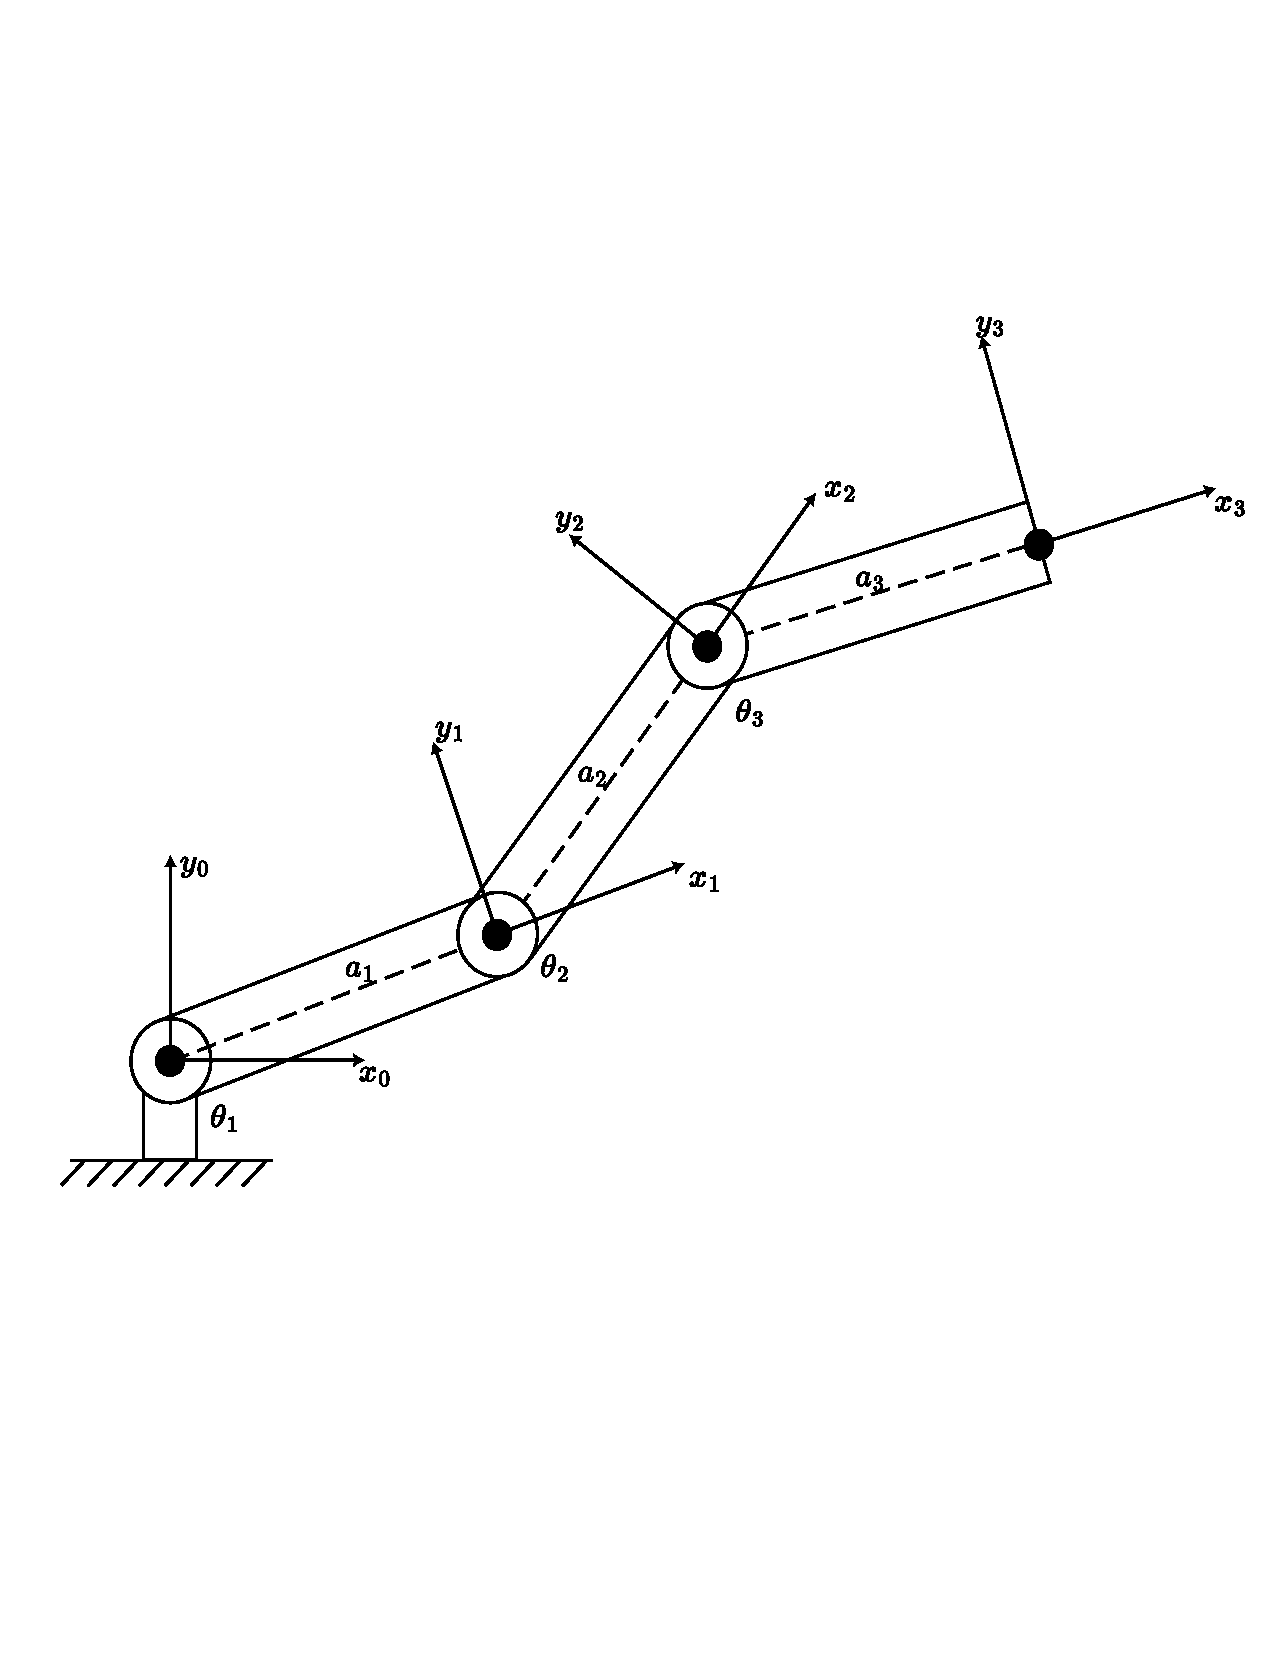
\includegraphics[width=0.8\linewidth]{Images/3r-planar.pdf}
    \caption{Braço planar do tipo 3R.}\label{fig:3r-planar-arm}
\end{figure}

\begin{equation}
    \mathbf{A}_i = \begin{bmatrix}
        c_i & -s_i & 0 & a_i c_i \\
        s_i & c_i  & 0 & a_i s_i \\
        0   & 0    & 1 & 0       \\
        0   & 0    & 0 & 1
    \end{bmatrix}
\end{equation}

Já para as matrizes \(T^0_i\), utilizamos a equação~\ref{eq:fkine}:

\begin{equation}
    \mathbf{T}^0_1 = \mathbf{A}_1
\end{equation}

\begin{equation}
    \mathbf{T}^0_2 = \mathbf{A}_1 \cdot \mathbf{A}_2 = \begin{bmatrix}
        c_{12} & -s_{12} & 0 & a_1c_1 + a_2c_{12} \\
        s_{12} & c_{12}  & 0 & a_1s_1 + a_2s_{12} \\
        0      & 0       & 1 & 0                  \\
        0      & 0       & 0 & 1
    \end{bmatrix}
\end{equation}

\begin{equation}
    \mathbf{T}^0_3 = \mathbf{A}_1 \cdot \mathbf{A}_2 \cdot \mathbf{A}_3 = \begin{bmatrix}
        c_{123} & -s_{123} & 0 & a_1c_1 + a_2c_{12} + a_3c_{123} \\
        s_{123} & c_{123}  & 0 & a_1s_1 + a_2s_{12} + a_3s_{123} \\
        0       & 0        & 1 & 0                               \\
        0       & 0        & 0 & 1
    \end{bmatrix}
\end{equation}

As três primeiras entradas da última coluna da matriz \(T^0_3\) dão a posição
\(\mathbf{P} = {\left[ x \ y \ z \right]}^{\top}\) do efetuador final em função
da configuração do manipulador. Note que $z = 0$ quaisquer que sejam os ângulos
das juntas pois, como esperado, o manipulador é planar. Além disso, analisando
a componente de rotação, fica evidente que a orientação do efetuador final com
relação ao frame da base é dada pela soma dos ângulos das juntas: $\psi =
    \theta_{123}$.

\section{Cinemática Diferencial}

Na seção anterior vimos como podemos estabelecer uma relação entre a
configuração de um manipulador com $n$ juntas com a pose do efetuador final no
espaço SE3. Nesta seção, iremos investigar de que forma se dá a relação de um
vetor de velocidades no espaço das juntas com a velocidade do efetuador final
no espaço de trabalho. Iremos ver que a matriz Jacobiana, atuando como uma
generalização da derivada para o caso multidimensional, é responsável por
estabelecer um mapeamento linear entre as velocidades e tem papel crucial na
caracterização da qualidade do movimento de um manipulador através da análise
das singularidades cinemáticas. Por fim, iremos analisar o problema da
cinemática inversa diferencial, uma aplicação direta do mapeamento estabelecido
pela matriz Jacobiana, proporcionando a geração eficiente de trajetórias
cartesianas (retilíneas) no espaço de trabalho do manipulador.

\subsection{A Jacobiana do Manipulador}

Dado um manipulador com $n$ juntas vamos considerar

\begin{equation}
    T_{n}^{0}(q) = \begin{bmatrix}
        R_{n}^{0}(q) & o_{n}^{0}(q) \\
        0            & 1
    \end{bmatrix}
\end{equation}

a transformação homogênea que expressa a pose do efetuador final com relação ao
\emph{frame} da base que, como já vimos, é função apenas da configuração \(q =
\begin{bmatrix}
    q_1 & \cdots & q_n
\end{bmatrix}^\top\).

Buscamos estabelecer relações da seguinte forma:

\begin{align}
    v_n^0 = J_v \dot{q} \\
    \omega_n^0 = J_\omega \dot{q}
\end{align}

onde \(v_n^0\) e \(\omega_n^0\) expressam respectivamente as velocidades linear
e angular do efetuador final e \(J_v\), \(J_\omega\) são matrizes de dimensão
\(3 \times n\). De maneira mais compacta, podemos escrever

\begin{equation}
    \xi = J \dot{q}
\end{equation}

onde teremos:

\begin{equation}
    \xi = \begin{bmatrix}
        v_n^0 \\
        \omega_n^0
    \end{bmatrix} \text{ e } J = \begin{bmatrix}
        J_v \\
        J_\omega
    \end{bmatrix}
\end{equation}

O vetor \(\xi\) de dimensão \(6 \times 1\) é denominado de velocidade do corpo
rígido (em inglês \emph{body velocity} ou \emph{twist}). Note também que a
matriz \(J\), chamada \emph{jacobiana do manipulador} ou simplesmente
jacobiana, é usualmente uma matriz de dimensão \(6 \times n\).

O cálculo da jacobiana, pode ser feito de maneira simples e sistemática ao
analisarmos as componentes angular e linear separadamente. No primeiro caso,
sabemos que a velocidade angular do efetuador final pode ser obtida através da
soma sucessiva das velocidades angulares de cada elo:

\begin{equation}\label{eq:angular-velocity}
    \omega_n^0 = \omega_{1}^0 + \omega_{2}^0 + \cdots + \omega_n^{0}
\end{equation}

Se a junta \(i\) é prismática não há rotação em torno do eixo \(z_{i-1}\) de
modo que \(\omega_i^{i-1} = 0\). Caso contrário, se a junta \(i\) é de
revolução a rotação dá se em torno do eixo $z_{i-1}$ com magnitude $\dot{q}_i$
de modo que:

\begin{equation}
    \omega_i^{0} = \dot{q_i} z_{i-1}^{0}
\end{equation}

onde obviamente teremos \(z_{0}^{0} = k = \begin{bmatrix}
    0 & 0 & 1
\end{bmatrix}^\top\)

A orientação do eixo \(z_{i}\) com relação ao \emph{frame} da base é dada por
\(z_{i}^0 = R_{i}^0 k\), então substituindo na equação
(\ref{eq:angular-velocity}) podemos escrever:

\begin{equation}
    \omega_n^0 = \rho_1 \dot{q_1} k + \rho_2 \dot{q_2} R_1^0 k + \cdots + \rho_n \dot{q_n} R_{n-1}^0 k
\end{equation}

onde \(\rho_i = 0\) se a junta \(i\) é prismática e \(\rho_i = 1\) caso
contrário. Fica claro então que a metade inferior da jacobiana é dada por:

\begin{equation}
    J_\omega = \begin{bmatrix}
        \rho_1 k & \rho_2 R_1^0 k & \cdots & \rho_n R_{n-1}^0 k
    \end{bmatrix}
\end{equation}

A metade superior da jacobiana é obtida calculando-se o vetor \(\dot{o}_n^0\).
Aplicando a regra da cadeia, temos:

\begin{equation}\label{eq:linear-velocity}
    \dot{o}_n^0 = \frac{\partial o_n^0}{\partial q_1} \dot{q_1} + \frac{\partial o_n^0}{\partial q_2} \dot{q_2} + \cdots + \frac{\partial o_n^0}{\partial q_n} \dot{q_n}
\end{equation}

onde fica claro que a i-ésima coluna de \(J_v\) é dada por:

\begin{equation}
    J_{v_i} = \frac{\partial o_n^0}{\partial q_i}
\end{equation}

Para obter a expressão de \(J_{v_i}\) vamos analisar novamente o caso de juntas
prismáticas e de revolução separadamente. No caso de uma única junta
prismática, então o efetuador final apresenta apenas translação ao longo do
eixo \(z_{i-1}\) de modo que:

\begin{equation}
    \dot{o}_n^0 = \dot{q_i} R_{i-1}^0 \begin{bmatrix}
        0 \\
        0 \\
        1
    \end{bmatrix} = \dot{q_i} z_{i-1}^0
\end{equation}

Comparando com a (\ref{eq:angular-velocity}) vemos que:

\begin{equation}
    J_{v_i} = z_{i-1}^0
\end{equation}

Já para o caso de uma junta de revolução, a velocidade linear do efetuador
final devido ao movimento do elo \(i\) é da forma \(\omega \times r\) dada pela
sua componente tangencial ao círculo de centro no ponto \(o_{i-1}\) e
extremidade no ponto \(o_n\) onde:

\begin{align*}
    \omega & = \dot{q_i} z_{i-1}^0 \\
    r      & = o_n^0 - o_{i-1}^0
\end{align*}

onde finalmente chegamos à expressão:

\begin{equation}
    J_{v_i} = z_{i-1}^0 \times (o_n^0 - o_{i-1}^0)
\end{equation}

Resumindo as equações obtidas acima, podemos calcular a jacobiana de qualquer
manipulador serial utilizando o seguinte procedimento:

A parte superior da matriz jacobiana \(J_v\) será:

\begin{equation}
    J_v = \begin{bmatrix}
        J_{v_1} & J_{v_2} & \cdots & J_{v_n}
    \end{bmatrix}
\end{equation}

onde a i-ésima coluna \(J_{v_i}\) é dada por:

\begin{equation}
    J_{v_i} =
    \begin{cases}
        z_{i-1}^0 \times (o_n^0 - o_{i-1}^0) & \text{se a junta $i$ é de revolução} \\
        z_{i-1}                              & \text{se a junta $i$ é prismática}   \\
    \end{cases}
\end{equation}

Já a parte inferior da matriz jacobiana \(J_\omega\) será:

\begin{equation}
    J_\omega = \begin{bmatrix}
        J_{\omega_1} & J_{\omega_2} & \cdots & J_{\omega_n}
    \end{bmatrix}
\end{equation}

onde a i-ésima coluna \(J_{\omega_i}\) é dada por:

\begin{equation}
    J_{\omega_i} =
    \begin{cases}
        z_{i-1}^0 & \text{se a junta $i$ é de revolução} \\
        0         & \text{se a junta $i$ é prismática}   \\
    \end{cases}
\end{equation}

Note que o cálculo da jacobiana torna-se possível apenas com o conhecimento da
função de cinemática direta \(T_n^0\) mostrando-se uma maneira eficiente para calcular 
não so a velocidade do efetuador final mas também a velocidade de qualquer ponto da 
estrutura cinemática do manipulador.

Como exemplo, considere o manipulador planar 3R introduzido na seção anterior.
Com base no procedimento descrito acima, a jacobiana do manipulador é dada por:

\begin{equation}
    J(q) = \begin{bmatrix}
        z_0^0 \times (o_3^0 - o_0^0) & z_1^0 \times (o_3^0 - o_1^0) & z_2^0 \times (o_3^0 - o_2^0) \\
        z_0^0                        & z_1^0                        & z_2^0
    \end{bmatrix}
\end{equation}

onde as termos envolvidos são:

\begin{align*}
    o_0^0 = \begin{bmatrix}
                0 \\
                0 \\
                0
            \end{bmatrix} \ \ o_1^0 = \begin{bmatrix}
                                          a_1 c_1 \\
                                          a_1 s_1 \\
                                          0
                                      \end{bmatrix} \ \ o_2^0 & = \begin{bmatrix}
                                                                      a_1 c_1 + a_2 c_{12} \\
                                                                      a_1 s_1 + a_2 s_{12} \\
                                                                      0
                                                                  \end{bmatrix} \ \ o_3^0 = \begin{bmatrix}
                                                                                                a_1 c_1 + a_2 c_{12} + a_3 c_{123} \\
                                                                                                a_1 s_1 + a_2 s_{12} + a_3 s_{123} \\
                                                                                                0
                                                                                            \end{bmatrix} \\
    z_0^0                                     & = z_1^0 = z_2^0 = \begin{bmatrix}
                                                                      0 \\
                                                                      0 \\
                                                                      1
                                                                  \end{bmatrix}
\end{align*}

Desenvolvendo as expressões acima, obtemos:

\begin{equation}
    J(q) = \begin{bmatrix}
        -a_1 s_1 - a_2 s_{12} - a_3 s_{123} & -a_2 s_{12} - a_3 s_{123} & -a_3 s_{123} \\
        a_1 c_1 + a_2 c_{12} + a_3 c_{123}  & a_2 c_{12} + a_3 c_{123}  & a_3 c_{123}  \\
        0                                   & 0                         & 0            \\
        0                                   & 0                         & 0            \\
        0                                   & 0                         & 0            \\
        1                                   & 1                         & 1            \\
    \end{bmatrix}
\end{equation}

Note que o manipulador planar não provoca qualquer translação ao longo do eixo
\(z\) uma vez que qualquer contribuição de \(J_{v_i}\) é nula na terceira
componente. Além disso, a única componente de rotação influenciada pelo
movimento das juntas é a rotação em torno também do eixo do eixo \(z\)
evidenciado pela terceira componente de \(J_{\omega_i}\) igual a 1.

\subsection{Singularidades}

A matriz jacobiana, de dimensão \(6 \times n\), estabelece o mapeamento linear
entre as velocidades das juntas e do efetuador final através da relação:

\begin{equation}\label{eq:jacobian-mapping}
    \xi = J(q) \dot{q}
\end{equation}

que coloca de forma explícita a dependência da configuração atual do
manipulador no cálculo de \(J\). Tal mapeamento implica que qualquer vetor de
velocidades do efetuador final é uma combinação linear das colunas da matriz
jacobiana:

\begin{equation}
    \xi = J_1 \dot{q_1} + J_2 \dot{q_2} + \cdots + J_n \dot{q_n}
\end{equation}

Uma vez que \(\xi \in \mathbb{R}^6\) o manipulador so conseguirá desempenhar
uma velocidade arbitrária se todas as colunas de \(J\) forem linearmente
independentes, ou seja, quando o posto da matriz jacobiana for igual a \(6\).
Para uma matriz \(J \in \mathbb{R}^{6 \times n}\) é sempre verdade que
\(\text{posto}(J) \leq \min(6, n)\). Com efeito, no caso do manipulador planar
3R tínhamos \(n = 3\) e desse modo \(\text{posto}(J) \leq 3\) evidenciando o
fato de que o manipulador não consegue desenvolver qualquer velocidade no
espaço de trabalho.

Configurações paras as quais o posto da matriz jacobiana é menor que o máximo
possível (em inglês \emph{rank deficiency}) são denominadas de
\emph{singularidades} ou configurações singulares. Identificar configurações
singulares é de grande importância para o controle de manipuladores por
diversos motivos, entre eles:

\begin{itemize}
    \item Singularidades representam configurações nas quais a mobilidade do manipulador
          é reduzida, ou seja, não é possível impor um movimento arbitrário ao efetuador
          final.
    \item Quando o manipulador está em uma singularidade, pode haver infinitas soluções
          para o problema de cinemática inversa.
    \item Nas proximidades de uma singularidade, pequenas variações nas velocidades no
          espaço operacional podem causar velocidades ilimitadas no espaço das juntas.
\end{itemize}

Quando a matriz jacobiana é quadrada, podemos usar o fato de que seu
determinante se anula em configurações singulares, contudo ainda assim o
problema de determinar o conjunto de configurações é difícil, pois precisamos
resolver a equação

\begin{equation}
    \det(J(q)) = 0
\end{equation}

que geralmente envolve termos com alto grau de não linearidade. Nas próximas
seções, examinaremos técnicas que viabilizam um esquema de controle capaz de se
afastar de configurações singulares ao explorar a redundância presente em
manipuladores planares. Isso se refere a casos em que a matriz Jacobiana é
retangular, apresentando mais velocidades no espaço das juntas (colunas) do que
velocidades possíveis no espaço de trabalho (linhas).

\subsection{Cinemática Inversa Diferencial}

Se a matriz jacobiana definida na equação (\ref{eq:jacobian-mapping}) é
quadrada e não singular, podemos resolver o problema de cinemática inversa
através da simples inversão da mesma:

\begin{equation}\label{eq:resolved-rate}
    \dot{q} = J^{-1}(q) \xi
\end{equation}

Se a configuração inicial do manipulador \(q(0)\) é conhecida as posições das
juntas podem ser calculadas integrando as velocidades no tempo:

\begin{equation}
    q(t) = q(0) + \int_{0}^{t} \dot{q}(\tau) d\tau
\end{equation}

A integração em tempo discreto pode ser feita utilizando técnicas de métodos
numéricos. A abordagem mais simples consiste na integração pelo método de
Euler, onde as posições das juntas no instante atual \(t_k\) são utilizadas
para calcular a configuração do manipulador no instante posterior \(t_{k+1} =
t_k + \Delta t\):

\begin{align}
    q(t_{k + 1}) & = q(t_k) + \dot{q}(t_k) \delta_t
\end{align}

onde \(\delta_t\) é um intervalo de integração apropriado (tempo de
amostragem).

O esquema de controle descrito acima é conhecido como \emph{resolved rate
    control}, o qual consegue de maneira simples e elegante o solucionar o problema
de gerar movimentos no efetuador final de velocidade constante sem recorrer à
soluções numéricas ou analíticas para o cálculo da cinemática inversa~\cite{corke_robotics_2023}. 
Tal esquema é útil na geração de trajetórias retilíneas no espaço de trabalho,
conhecidas como trajetórias cartesianas, uma vez que a componente translacional
da velocidade do efetuador final tem direção constante ao longo de todo o
trajeto pode ser tratada de maneira independente da componente rotacional.

Como exemplo, ainda considerando o manipulador planar 3R, poderíamos apenas
especificar um vetor de velocidades \(\xi\) que leva em conta as componentes do
plano \(xy\) da velocidade linear e a componente de rotação angular em torno do
eixo \(z\) de modo que:

\begin{equation}
    \xi = \begin{bmatrix}
        v_x \\
        v_y \\
        \omega_z
    \end{bmatrix}
\end{equation}

Assim a matriz jacobiana se torna livre das linhas que possuem apenas zeros:

\begin{equation}
    J(q) = \begin{bmatrix}
        -a_1 s_1 - a_2 s_{12} - a_3 s_{123} & -a_2 s_{12} - a_3 s_{123} & -a_3 s_{123} \\
        a_1 c_1 + a_2 c_{12} + a_3 c_{123}  & a_2 c_{12} + a_3 c_{123}  & a_3 c_{123}  \\
        1                                   & 1                         & 1
    \end{bmatrix}
\end{equation}

e contanto que não seja singular pode ser facilmente invertida. Desse modo, se
quisermos por exemplo, gerar um movimento retilíneo no efetuador final paralelo
ao eixo \(x\) do plano \(xy\) com velocidade constante, basta tomar \(\xi = \begin{bmatrix}
    v_x & 0 & 0
\end{bmatrix}^\top\).

\section{Manipuladores redundantes}

Manipuladores cinematicamente redundantes, são aqueles que possuem mais juntas
do que o número estritamente necessário para a execução de uma determinada
tarefa. Este excedente de juntas confere a esses manipuladores um nível
aumentado de destreza, permitindo-lhes navegar em ambientes complexos com maior
flexibilidade. Nesta seção vamos introduzir uma solução geral para o problema
da cinemática inversa diferencial quando o matriz jacobiana é retangular,
envolvendo o conceito da sua \emph{pseudo-inversa}. Em seguida, utilizando a
decomposição em valores singulares de \(J\) iremos fornecer uma descrição
geométrica e qualitativa da destreza associada à uma dada configuração através
dos conceitos do elipsoide e da medida de manipulabilidade. Por fim, vamos ver
como podemos utilizar a solução geral fornecida pela pseudo-inversa para
otimizar diferentes índices de performance com o objetivo de evitar
singularidades e limites mecânicos das juntas.

\subsection{Pseudo-Inversa da Jacobiana}

Num manipulador cinematicamente redundante, a matriz jacobiana de dimensão \(m
\times n\) será retangular (\(m < n\)). Isso significa que \(J\) possui mais
colunas do que linhas e nesse caso existem infinitas soluções para o problema
de cinemática inversa diferencial. Uma solução viável é formular o problema como 
um de otimização linear com restrições, onde a solução ótima é obtida minimizando 
o custo quadrático das velocidades das juntas~\cite{siciliano_robotics_2009}:

\begin{equation}
    \min_{\dot{q}} \left\Vert \dot{q} \right\Vert^2 \text{ sujeito a } J \dot{q} = \xi
\end{equation}

Pode ser mostrado que nesse caso, a solução ótima é dada por:

\begin{equation}\label{eq:pseudo-inverse}
    \dot{q} = J^\dag \xi + (I_n - J^\dag J) \dot{q_0}
\end{equation}

onde \(\dot{q_0}\) é um vetor de velocidades arbitrário e a matriz \(J^\dag\) é
conhecida como \emph{matriz inversa de Moore-Penrose} ou apenas
\emph{pseudo-inversa} de \(J\) e é dada por:

\begin{equation}
    J^\dag = J^\top {(J J^\top)}^{-1}
\end{equation}

Vale notar que o termo \(I_n - J^\dag J\) atua projetando o vetor \(\dot{q_0}\)
no espaço nulo de \(J\). Com efeito, aplicando a jacobiana à esquerda na
equação (\ref{eq:pseudo-inverse}) temos:

\begin{align*}
    J \dot{q} & = J J^\dag \xi + J (I_n - J^\dag J) \dot{q_0}                                   \\
              & = J J^\top {(J J^\top)}^{-1} \xi + (J - J J^\top {(J J^\top)}^{-1} J) \dot{q_0} \\
              & = \xi + (J - J) \dot{q_0}                                                       \\
    J \dot{q} & = \xi
\end{align*}

permitindo que o manipulador realize movimentos internos no espaço das juntas
que que não afetam a velocidade \(\xi\) do efetuador final.

\subsection{Medida de Manipulabilidade}

Uma maneira de investigar mais a fundo o mapeamento linear estabelecido pela
jacobiana é entender como a mesma ``deforma'' o vetor \(\dot{q}\) de entradas
para produzir o vetor \(\xi\) de saídas. Para isso, podemos considerar o disco
formado pelo conjunto de velocidades com norma unitária:

\begin{equation}
    \left\Vert \dot{q} \right\Vert^2 = q_1^2 + q_2^2 + \cdots + q_n^2 \leq 1
\end{equation}

Substituindo a solução de menor norma \(\dot{q} = J^\dag \xi\):

\begin{align}\label{eq:manipulability-ellipsoid}
    \left\Vert \dot{q} \right\Vert^2 & = \dot{q}^\top \dot{q} \notag                                                    \\
                                     & = {(J^\dag \xi)}^\top J^\dag \xi \notag                                          \\
                                     & = \xi^\top {(J^\top {(J J^\top)}^{-1})}^\top J^\top {(J J^\top)}^{-1} \xi \notag \\
                                     & = \xi^\top {(J J^\top)}^{-1} (J J^\top) {(J J^\top)}^{-1} \xi \notag             \\
    \left\Vert \dot{q} \right\Vert^2 & = \xi^\top {(J J^\top)}^{-1} \xi \leq 1
\end{align}

A equação (\ref{eq:manipulability-ellipsoid}) define uma região no espaço de
trabalho conhecido como \emph{elipsoide de manipulabilidade} que representa
todas as velocidades possíveis do efetuador final para uma dada configuração do
manipulador. Esse fato pode ser facilmente verificado ao considerarmos a
decomposição em valores singulares (SVD) da jacobiana \(J = U \Sigma V^\top\):

\begin{align}\label{eq:manipulability-ellipsoid-svd}
    \left\Vert \dot{q} \right\Vert^2 & = \xi^\top {(U \Sigma V^\top V \Sigma^\top U^\top)}^{-1} \xi \notag \\
                                     & = \xi^\top {(U \Sigma^2 U^\top)}^{-1} \xi \notag                    \\
                                     & = \xi^\top U \Sigma^{-2} U^\top \xi \notag                          \\
    \left\Vert \dot{q} \right\Vert^2 & = {(U^\top \xi)}^\top \Sigma^{-2} (U^\top \xi)
\end{align}

onde sabemos que \(U\) e \(V\) são matrizes ortogonais, isto é \(U^{-1} =
U^\top\) e \(V^{-1} = V^\top\). Além disso a matriz

\begin{equation}
    \Sigma^{-2} = \begin{bmatrix}
        \sigma_1^{-2} &               &        &               & \\
                      & \sigma_2^{-2} &        &               & \\
                      &               & \ddots &               & \\
                      &               &        & \sigma_m^{-2} & \\
    \end{bmatrix}
\end{equation}

é diagonal e os termos que \(\sigma_1 \geq \sigma_2 \geq \cdots \geq \sigma_m\) são os valores
singulares de \(J\). Por fim, ao fazermos a substituição \(w = U^\top \xi\) podemos reescrever a equação
(\ref{eq:manipulability-ellipsoid-svd}) como:

\begin{equation}
    w^\top \Sigma^{-2} w = \sum_{i=1}^m{\frac{{w_i}^2}{{\sigma_i}^2}} \leq 1
\end{equation}

evidenciado que o disco é mapeado num elipsoide com eixos alinhados a um
sistema de coordenadas rotacionado por \(U^\top\). No sistema de coordenadas
original, os semi-eixos do elipsoide são dados pelos vetores \(\sigma_i u_i\).

A medida de manipulabilidade \(\mu\) é definida como o produto dos valores
singulares de \(J\):

\begin{equation}\label{eq:manipulability}
    \mu = \sigma_1 \sigma_2 \cdots \sigma_m
\end{equation}

que é proporcional ao volume do elipsoide de manipulabilidade. Ao passo que nos
aproximamos de uma singularidade, um ou mais dos valores singulares de \(J\) se
aproximam de zero, reduzindo o volume do elipsoide e consequentemente a
destreza do manipulador. Isso pode ser visualizado na
figura~\ref{fig:manipulability-ellipsoid} onde para o braço planar 3R, o
elipsoide de manipulabilidade é mostrado para diferentes configurações do
manipulador e vai se tornando cada vez mais achatado à medida que nos
aproximamos do limite do espaço de trabalho.

\begin{figure}
    \centering
    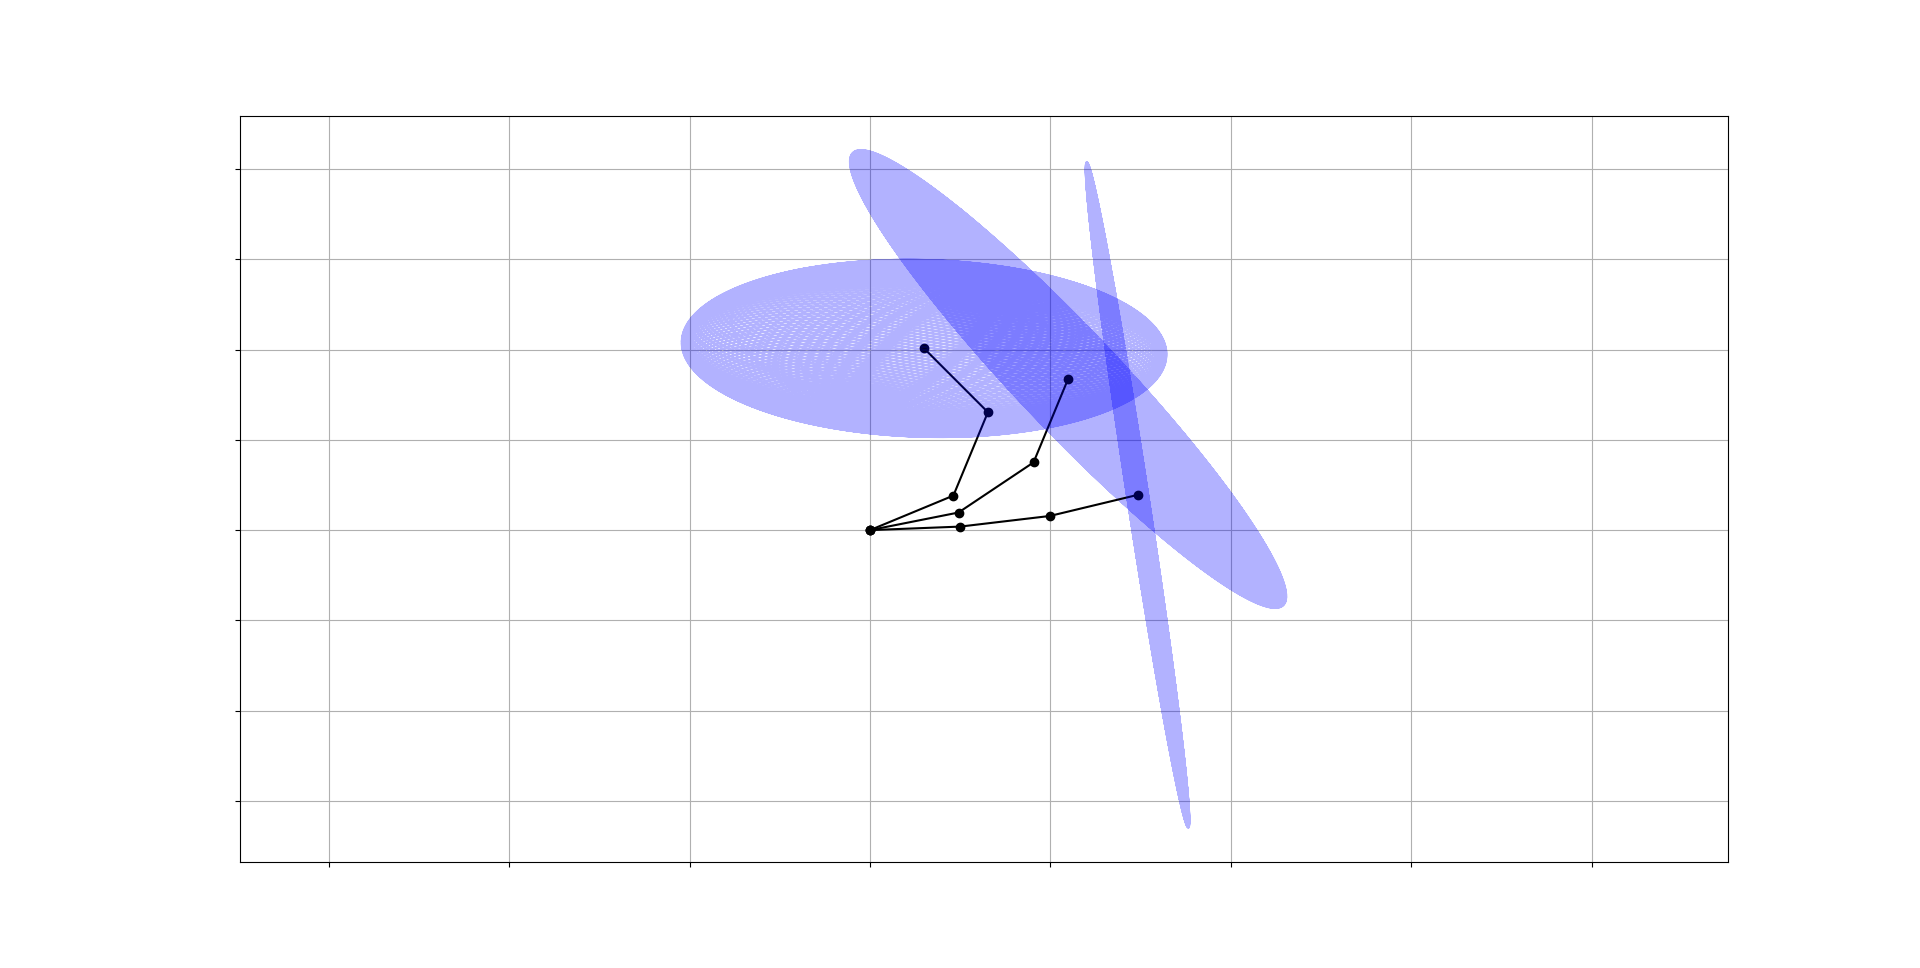
\includegraphics[width=0.9\textwidth]{Images/3r-ellipsoid.png}
    \caption{Elipsoide de manipulabilidade para diferentes configurações do manipulador planar 3R.}\label{fig:manipulability-ellipsoid}
\end{figure}

\subsection{Resolução de Redundância}

Ao estabelecermos a solução geral dada pela equação (\ref{eq:pseudo-inverse}),
dissemos que o vetor \(\dot{q_0}\) pode ser escolhido arbitrariamente. Uma
possibilidade é tomá-lo de forma a maximar algum índice de performance \(w\),
para isso escolhendo o vetor na direção do gradiente:

\begin{equation}\label{eq:metric-gradient}
    \dot{q_0} = k_0 {\left( \frac{\partial w(q)}{\partial q} \right)}^\top
\end{equation}

onde \(k_0 > 0\) é uma constante positiva que determina o tamanho do passo.

Uma escolha natural para o índice de performance \(w\) é a \emph{medida de
    manipulabilidade de Yoshikawa}:

\begin{equation}\label{eq:yoshikawa}
    w(q) = \sqrt{\det(J(q){J(q)}^\top)}
\end{equation}

onde vale ressaltar que é equivalente àquela definida na a equação
(\ref{eq:manipulability}) uma vez que se \(\lambda_i\) são os autovalores de
\(J J^\top\) então \(\sigma_i = \sqrt{\lambda_i}\).

Uma alternativa ao cálculo da \ref{eq:yoshikawa} é utilizar uma métrica mais simples como a
\emph{distância para os limites mecânicos das juntas} dada por:

\begin{equation}
    w(q) = -\frac{1}{2n} \sum_{i=1}^{n}{{\left(\frac{q_i - \bar{q_i}}{q_{iM} - q_{im}}\right)}^2}
\end{equation}

Ao maximar tal índice, espera-se que o manipulador mantenha-se próximo ao ponto
central de atuação de cada junta, evitando assim configurações singulares no
limite do espaço de trabalho. Além disso, o vetor gradiente pode ser calculado
de maneira analítica onde cada coordenada é dada por:

\begin{equation}\label{eq:joint-distance-grad}
    \frac{\partial w(q)}{\partial q_i} = -\frac{1}{n} \frac{q_i - \bar{q_i}}{{(q_{iM} - q_{im})}^2}
\end{equation}

Outro ponto a salientar é que a escolha do tamanho do passo \(k_0\) é crucial
para a performance do algoritmo~\cite{siciliano_springer_2008}. Se \(k_0\) 
for muito pequeno o processo de otimização pode se tornar muito lento, enquanto 
que se \(k_0\) for muito grande isso pode a uma diminuição ou até
 mesmo não convergência do valor de \(w\) devido a oscilações em torno do ponto 
 de máximo local.

No próximo capítulo, iremos aplicar os conceitos apresentados até agora na
conecepção de um ambiente simulado para um manipulador redundante com cinco
graus de liberdade. O objetivo principal será a execução de trajetórias
retilíneas no espaço de trabalho \(\mathcal{T} \in \text{SE}(3)\) que levam
apenas em consideração a posição do efetuador e com isso explorar a resolução
de redundância para otimizar diferentes índices relacionados a configuração do
manipulador durante a execução da trajetória.

\cleardoublepage{}
% % % % % % % % % % % % % % % % % % % % % % % % % % %
\chapter{Implementação}\label{cap:methods}

Neste capítulo, iremos explorar as ferramentas e métodos utilizados na
concepção de um ambiente robótico simulado para um manipulador com cinco graus
de liberdade do tipo 5R. O manipulador tem uma cadeia cinemática simples que
pode ser entendida como a composição de dois outros braços planares, mas que
permite que a posição do efetuador final não esteja limitada, por exemplo, a um
plano de altura constante. Começaremos explorando a modelagem da cadeia
cinemática e também a representação do modelo virtual do robô dentro do
simulador \emph{Webots}. Em seguida, iremos definir a arquitetura de
comunicação proposta para se controlar o manipulador utilizando o conceito de
\emph{Actions} presente no framework \emph{Robot Operating System} (ROS), o
qual permitiu uma implementação modularizada para execução dos experimentos.
Por fim, iremos detalhar o esquema de controle e bibliotecas utilizadas na
implementação do algoritmo RRMC para execução de trajetórias retilíneas bem como os 
experimentos realizados para se avaliar a resolução de redundância na execução de 
tais trajetórias.

\section{Simulação de manipuladores robóticos}

Simuladores de física tornam possível a pesquisa e desenvolvimento na robótica,
pois permitem que os pesquisadores testem e validem métodos teóricos
inicialmente ou exclusivamente em um simulador, uma vez que os robôs em si são
frequentemente caros, frágeis e escassos~\cite{robotic_applications}. Os
simuladores oferecem um ambiente acessível e barato de prototipação com uma
variedade de robôs disponíveis e prontos para uso, sem o risco de danificar o
equipamento físico economizando assim tempo e recursos. A simulação pode ser
executada mais rápido do que em tempo real (o que é especialmente importante
para abordagens baseadas em aprendizado ou análises de natureza estatística), é
paralelizável e não requer intervenção física para reiniciar um ambiente.

Para se implementar um ambiente simulado diversas características do simulador
devem ser levadas em conta, tais como: o modelo do robô a ser simulado, os
sensores e atuadores disponíveis, o ambiente físico a ser simulado (por
exemplo, correntes de ar, ambientes aquáticos), linguagens de programação
disponíveis para controle do robô, formatos suportados, extensibilidade,
documentação entre outros.

Neste trabalho, optamos por utilizar a linguagem de programação \emph{Python}
devido à disponibilidade de pacotes para computação numérica e visualização
(\emph{Numpy, Pandas e Matplotlib}) bem como voltadas exclusivamente para a
aplicações relacionadas à robótica como \emph{Robotics Toolbox for
    Python}~\cite{rtb}. O simulador escolhido foi o Webots~\cite{webots} devido a
possibilidade de prototipar o modelo virtual do manipulador do zero aliado a
testes rápidos de diversos designs. Além disso, o Webots oferece suporte
oficial ao ROS, o que permitiu a implementação de um sistema modularizado, onde
cada componente executa uma tarefa específica, facilitando a manutenção e a
extensão do mesmo, inclusive para o interfaceamento com um robô real.

\begin{figure}
    \centering
    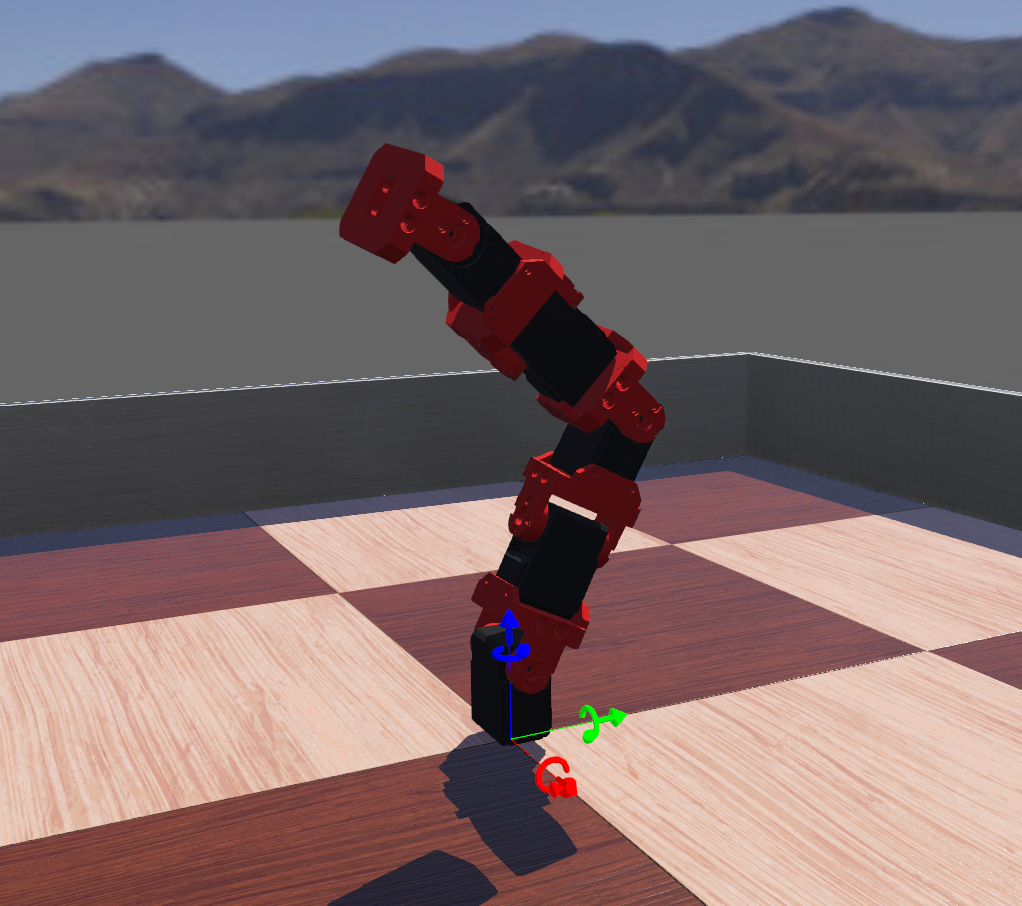
\includegraphics[width=0.8\textwidth]{./Images/webots-robot.png}
    \caption{Modelo virtual do manipulador no Webots.}\label{fig:robot-model}
\end{figure}

\subsection*{Modelagem da Cadeia Cinemática}

A estrutura cinemática do manipulador 5R foi pensada de modo a ser uma simples
cadeia de juntas rotacionais, permitindo uma fácil construção do robô real,
como por exemplo, sendo composto por uma sequência de servo motores conectados
por soquetes como ilustrado na figura~\ref{fig:robot-model}. A cadeia
cinemática é similar ao que já vimos no exemplo dos braço planar 3R, contudo
juntas consecutivas possuem eixos de rotação ortogonais entre si. Com isso, a
posição do efetuador final não fica restrita a um plano perpendicular ao eixo
de rotação das juntas, o que permite especificarmos no espaço de trabalho,
vetores com três coordenadas para compor a trajetória a ser seguida. Como \(n =
5 \text{ e } m = 3\) o manipulador tem grau de redundância de duas juntas
excedentes. A tabela~\ref{tab:dh-parameters-5r} resume os parâmetros DH
utilizados para modelar a cadeia cinemática.

\begin{table}[htbp]
    \centering
    \begin{tabular}{c c c c c c}
        \toprule
        \textbf{Elo} & \(\theta\)   & \(d\) & \(a\) & \(\alpha\)   \\
        \midrule
        1            & \(\theta_1\) & 0     & 0.06  & \(\pi / 2\)  \\
        2            & \(\theta_2\) & 0     & 0.06  & \(-\pi / 2\) \\
        3            & \(\theta_3\) & 0     & 0.06  & \(\pi / 2\)  \\
        4            & \(\theta_4\) & 0     & 0.06  & \(-\pi / 2\) \\
        5            & \(\theta_5\) & 0     & 0.02  & \(\pi / 2\)  \\
        \bottomrule
    \end{tabular}
    \caption{Parâmetros DH para o manipulador 5R.}\label{tab:dh-parameters-5r}
\end{table}

A fixação de frames imposta pela convenção DH nem sempre permite que o frame da
base do manipulador coincida com o frame do mundo, introduzindo nesse caso a
utilização de \emph{offsets} nos parâmetros variáveis das juntas, ou
transformações fixas entre os frames que não mudam conforme as juntas são
atuadas. Optamos por adotar uma abordagem mais direta, onde introduzimos a
transformação \(\mathbf{T}^{w}_0\) que relaciona o frame do mundo \(\{w\}\) com
o frame da base do manipulador \(\{0\}\):

\begin{equation}
    \mathbf{T}^{w}_0 = Trans_z(0.04) \cdot Rot_z(\pi) \cdot Rot_y(\pi / 2)
\end{equation}

Assim, para se calcular a cinemática direta do manipulador, prosseguimos de
maneira usual na cadeia cinemática adicionando a transformação
\(\mathbf{T}^{w}_0\) ao início da multiplicação matricial:

\begin{equation}
    \mathbf{T}^{w}_5 = \mathbf{T}^{w}_0 \cdot \mathbf{T}^{0}_1 \cdot \mathbf{T}^{1}_2 \cdot \mathbf{T}^{2}_3 \cdot \mathbf{T}^{3}_4 \cdot \mathbf{T}^{4}_5
\end{equation}

Por outro lado, durante a etapa da cinemática inversa diferencial, precisamos
especificar vetores livres \(\xi^w\) que indicam a velocidade cartesiana do
efetuador no mundo em termos do frame da base do manipulador. Para isso,
utilizamos a matriz de rotação da transformação inversa (do frame \(\{0\} \to
\{w\}\)), isto é:

\begin{equation}
    \xi^0 = {Rot(\mathbf{T}^w_0)}^\top \xi^w
\end{equation}

\begin{figure}
    \centering
    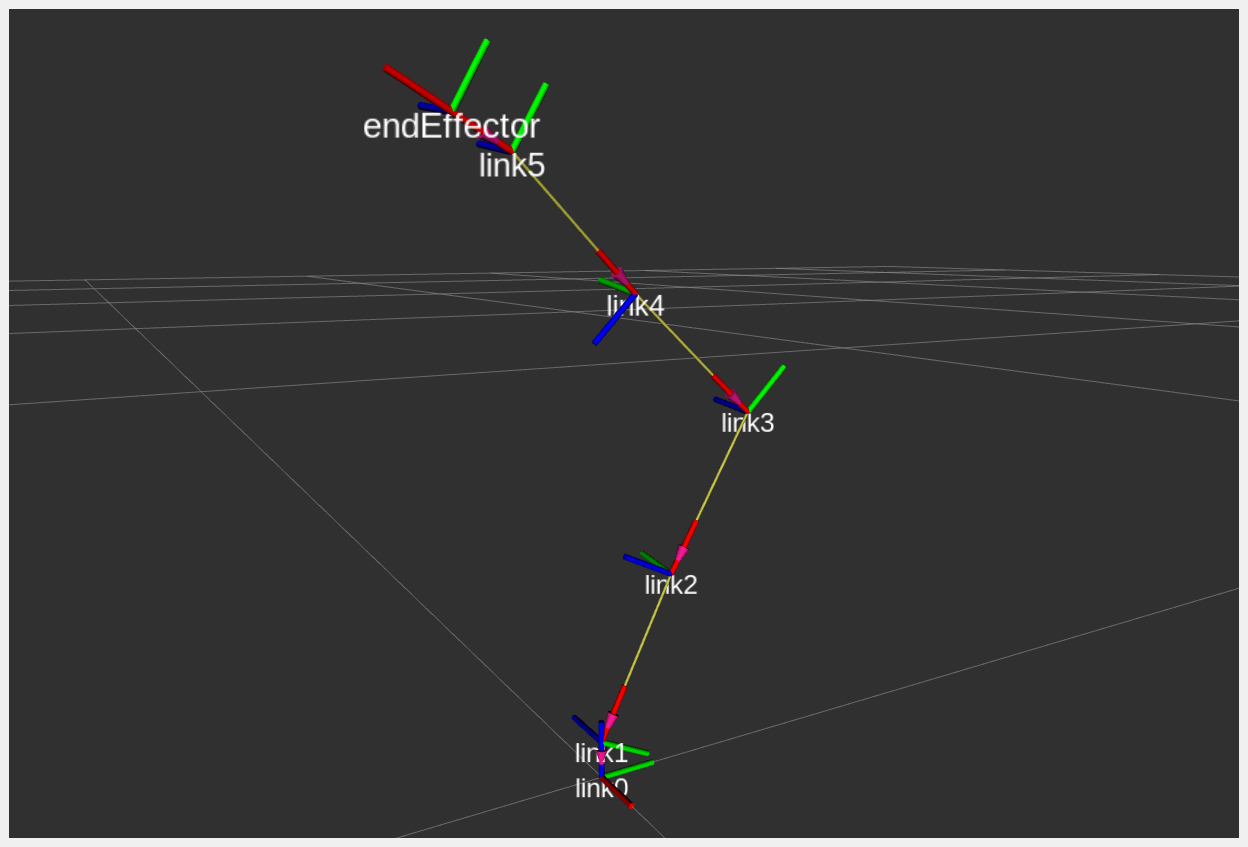
\includegraphics[width=0.8\textwidth]{./Images/rviz-chain.png}
    \caption{Cadeia cinemática visualizada no RViz.}\label{fig:kin-chain}
\end{figure}

\subsection*{Modelo dinâmico do manipulador}

Com o intuito de conferir um caráter mais realista para a simulação, um modelo
dinâmico para o robô foi construído especificando as propriedades físicas e
geometrias de colisão de cada elo no simulador. A figura~\ref{fig:dyn-chain}
mostra as formas primitivas do tipo \emph{Box} (caixas) que foram usadas para
compor a geometria de cada par servo-soquete que compõe um elo da cadeia. Para
o simulador computar o modelo dinâmico ao longo do tempo, foram fornecidas as
informações de massa do servo-motor (disponível na especificação do fabricante)
e no caso dos soquetes, a densidade do material PLA foi utilizada para estimar
sua massa com base no volume da geometria modelada (conjunto de caixas). Além
disso, a definição das matrizes de inércia ficou por conta do próprio
simulador, que estima seu valor com base na massa fornecida e na posição e
orientação das primitivas utilizadas durante a modelagem. Vale ressaltar que a
adição das propriedades dinâmicas tem caráter apenas de aproximação de um cenário
mais real, tendo em vista que o esquema de controle proposto atua apenas na
velocidade das juntas ao passo que a posição do motor é controlada de maneira
automática pelo simulador através de um PID intrínseco à simulação de um
dispositivo como o motor.

\begin{figure}
    \centering
    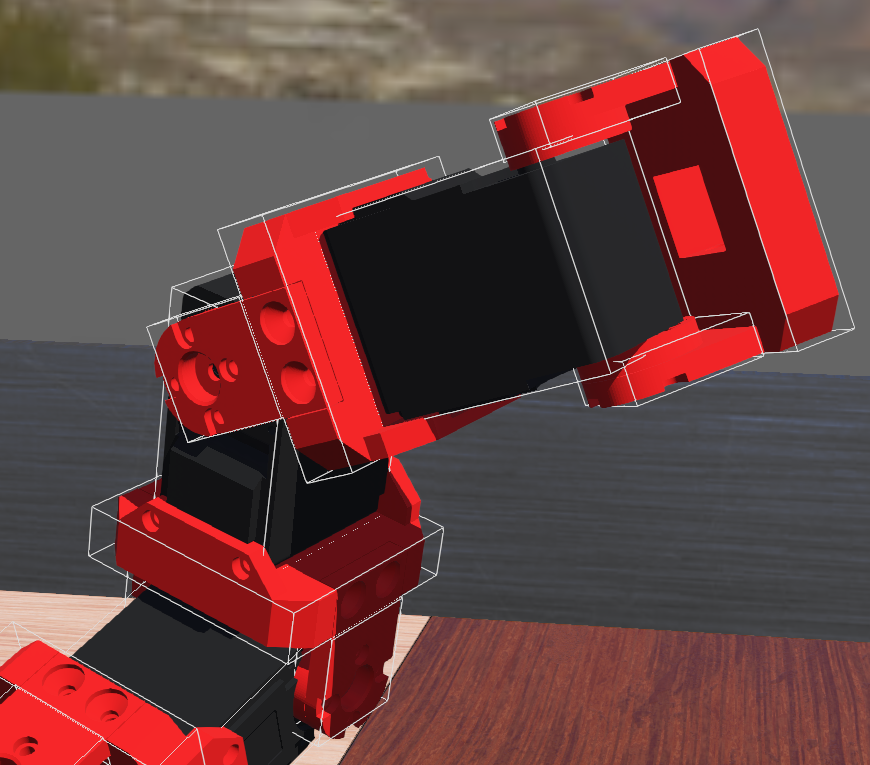
\includegraphics[width=0.6\textwidth]{./Images/dynamic-model.png}
    \caption{Geometria de colisão do modelo virtual do manipulador.}\label{fig:dyn-chain}
\end{figure}

\section{Arquitetura de comunicação}

A comunicação do controlador com o ambiente simulado do robô foi feita através
do uso do framework ROS, que consiste num conjunto de bibliotecas e pacotes de
software que facilitam a troca de mensagens entre diferentes componentes de um
sistema robótico. O próprio simulador Webots oferece suporte nativo ao ROS, com
uma documentação detalhada de como configurar um projeto e o uso básico de
troca de mensagens entre diferentes processos.

A arquitetura de comunicação do ROS é baseada em uma estrutura de grafo, onde
nós representam processos individuais que interagem com outros nós recebendo e
enviando mensagens, através de tópicos. Idealmente, um nó deve ser responsável
por uma única tarefa modular, como controlar os motores do robô ou enviar dados
coletados por um sensor de distância.

Os tópicos são os canais pelos quais os nós trocam mensagens e seguem um modelo
\emph{publisher/subscriber}, onde nós publicam mensagens em um tópico e outros
nós se inscrevem para receber essas mensagens, de maneira completamente
anônima. As mensagens passadas nos tópicos podem variar amplamente e geralmente
são definidas pelo usuário, cobrindo dados de sensores, comandos de controle de
motores, informações de estado, comandos de atuadores entre outros.

\subsection*{Serviços e Ações no ROS}

Serviços e ações constituem outras formas de comunicação entre nós no grafo do
ROS e implementam uma abordagem de troca de mensagens do tipo cliente/servidor.
Serviços representam ações que um nó pode executar com um início e fim
definidos, retornando um único resultado e são normalmente usados para tarefas
que possuem requisição e retorno, como por exemplo capturar uma imagem de um
único quadro, dispensando o processamento contínuo. Por outro lado, ações são
destinadas a tarefas de longa duração e são construídas com base em diferentes
tópicos e serviços. Ações consistem em três partes: um objetivo, um
\emph{feedback} e um resultado. Um nó do tipo cliente de ação envia um objetivo
para um nó servidor de ação, que reconhece a requisição, retorna um fluxo
continua de dados através de um feedback até que a ação seja concluída ou
cancelada, quando por fim retorna um resultado.

\begin{figure}
	\centering
	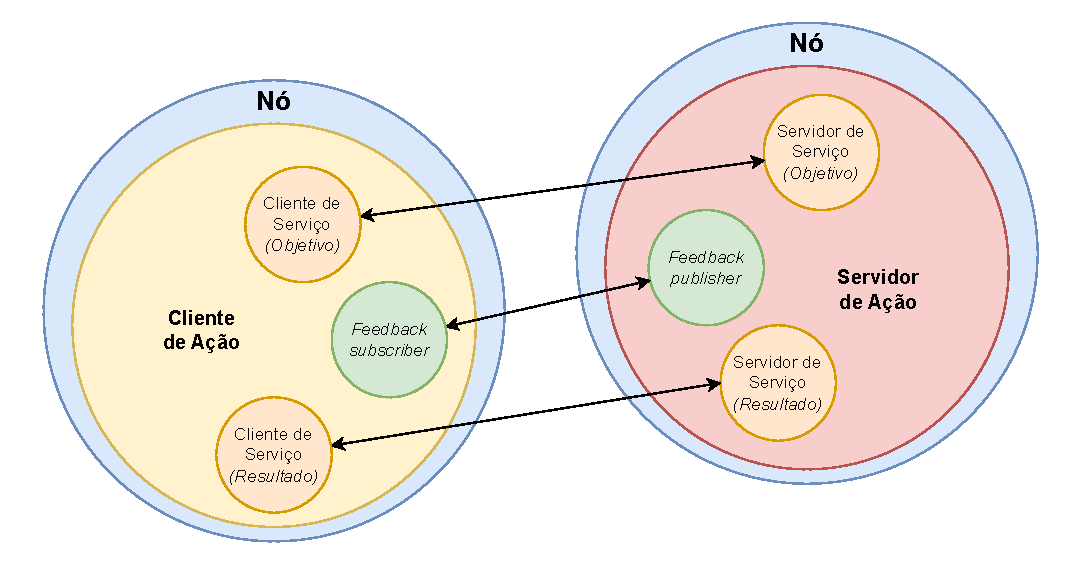
\includegraphics[width=0.8\textwidth]{./Images/ros-action.pdf}
	\caption{Componentes que constituem uma ação dentro do ROS. Adaptado de \cite[p. 36]{bassa_very_2023}.}\label{fig:ros-action}
\end{figure}

\subsection*{Grafo de comunicação no ROS}

Com o objetivo de se executar trajetórias no espaço de trabalho do manipulador,
a arquitetura de comunicação foi projetada de modo especificar um objetivo
através de uma ação do tipo \textbf{trajectory\_action} (nós
\emph{trajectory\_action\_server} e \emph{trajectory\_action\_client}) e
controlar o manipulador (nós \emph{snake\_driver} e \emph{snake\_controller}).
A arquitetura de comunicação proposta para o controle do manipulador é
ilustrada no grafo da figura~\ref{fig:coms_arch}, onde temos nós, tópicos e
ações associados a execução de uma trajetória. A seguir temos uma breve
descrição do funcionamento de cada nó.

\begin{itemize}
    \item \textbf{snake\_driver} {-} Nó instanciado pelo simulador, responsável por controlar os motores do manipulador.
          Está inscrito no tópico \texttt{target\_joint\_states} que recebe a configuração das juntas desejada para o manipulador
          e publica no tópico \texttt{joint\_states} os valores lidos pelos sensores de posição de cada motor. Este nó pode ser substituído por um nó
          que se comunique com um robô real, bastando que a interface de comunicação seja mantida, garantindo uma transferência natural do ambiente simulado para testes físicos.

    \item \textbf{snake\_controller} {-} Nó responsável por implementar a lógica de controle do manipulador. Este nó está inscrito/publica nos dois tópicos
          anteriores para interação com o \emph{driver} do manipulador. Além disso, se inscreve
          num tópico \texttt{rrc\_input}, recebendo parâmetros de controle do algoritmo~\ref{rrc-alg} e publica no tópico \texttt{rrc\_output} dados
          relativos à posição do efetuador final e métricas de desempenho.

    \item \textbf{trajectory\_action\_server} {-} Nó responsável por receber um objetivo de posição e informações do efetuador final para execução de uma trajetória
          no espaço de trabalho do manipulador, publicando no tópico \texttt{rrc\_input} os parâmetros de controle.

    \item \textbf{trajectory\_action\_client} {-} Nó responsável por enviar um objetivo de posição para o servidor de ação \texttt{trajectory\_action\_server} e
          receber o resultado da execução da trajetória. Através da interface de ação, o cliente recebe feedback do progresso da execução da trajetória e o resultado final,
          salvando todos os dados em um arquivo de \emph{log}, para posterior análise.
\end{itemize}

\begin{figure}
    \centering
    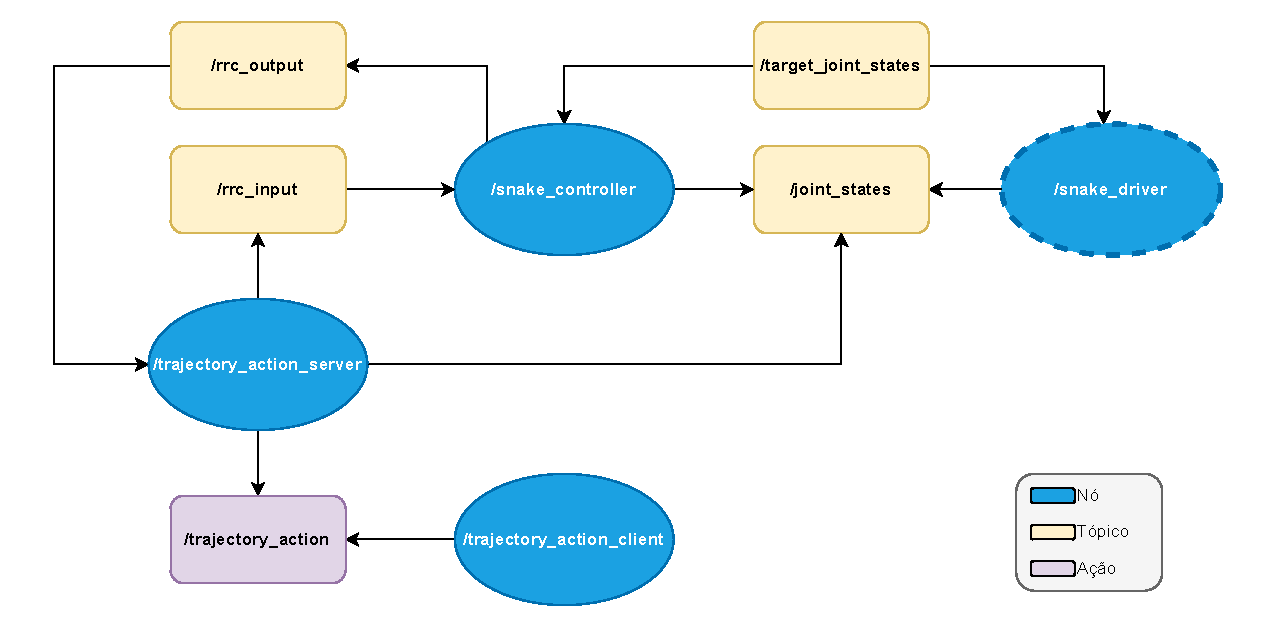
\includegraphics[width=0.8\textwidth]{./Images/ros-arch.pdf}
    \caption{Arquitetura de comunicação proposta para controle do manipulador.}\label{fig:coms_arch}
\end{figure}

\section{O Algoritmo \emph{Resolved Rate Motion Control}}

Para realizar o controle da trajetória do manipulador e também a resolução da
redundância, foi utilizado o esquema de controle \emph{Resolved Rate Motion Control} (RRMC)
definido no capítulo anterior. A figura~\ref{fig:block-diagram} ilustra o
diagrama de blocos do controlador RRMC implementado pelo nó
\emph{snake\_controller}. Dada uma taxa de variação da posição do efetuador
final \(\xi\) e um vetor de velocidades das juntas \(\dot{q_0}\), o controlador
atua atualizando a configuração do manipulador de acordo com a
equação~\ref{eq:pseudo-inverse}.

\begin{figure}
    \centering
    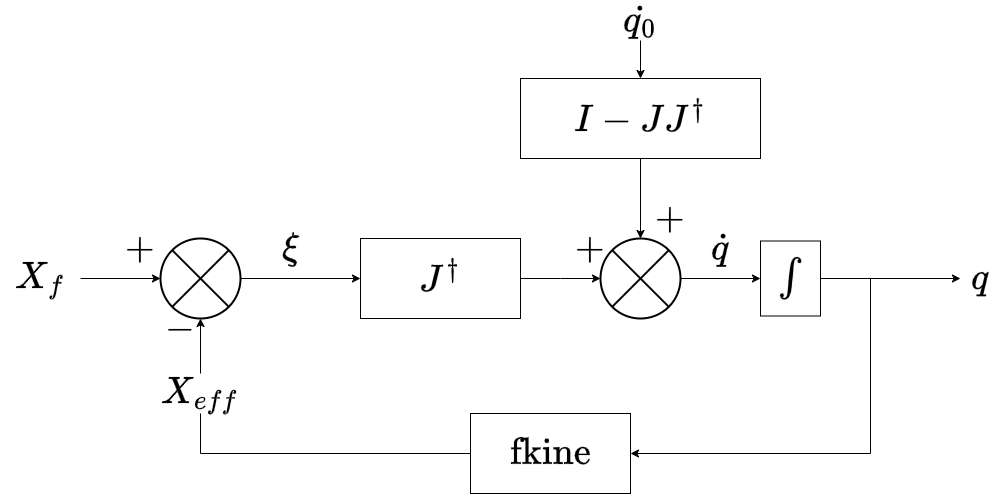
\includegraphics[width=0.6\textwidth]{./Images/control-scheme.png}
    \caption{Diagrama de blocos do controlador RRMC}\label{fig:block-diagram}
\end{figure}

Para a realização dos experimentos, foi implementado o algoritmo~\ref{rrc-alg}
(código disponível em \url{https://github.com/hugotallys/snakesim}) que escolhe o vetor \(\dot{q_0}\) de acordo com o gradiente dado pela
equação~\ref{eq:metric-gradient}. As duas métricas apresentadas anteriormente
foram calculadas: \emph{distância para os limites mecânicos das juntas} e
\emph{medida de manipulabilidade de Yoshikawa}. No primeiro caso, o gradiente é
calculado analiticamente de acordo com a equação~\ref{eq:joint-distance-grad}.
Já para a manipulabilidade, o gradiente é estimado numericamente através de
diferenças finitas, considerando um passo \(h\) suficientemente pequeno.

\begin{algorithm}
    \caption{\emph{Resolved Rate Motion Controller} {-} Atualizando o estado das juntas}\label{rrc-alg}
    \begin{algorithmic}[1]\Procedure{updateJointPosition}{$q$, $\xi$, $k_0$, $\delta_t$, \texttt{metricName}}
        \State$\xi \gets {Rot(\mathbf{T}^w_0)}^\top \xi$
        \State$J \gets Jacobian(q)$
        \State$J^\dag \gets J^\top {(J J^\top)}^{-1}$

        \State$n \gets length(q)$
        \State$\dot{q_0} \gets array(size: n)$

        \For{$i \gets 0 \ \texttt{to} \ n - 1$} \Comment{Calculando o gradiente da métrica}
        \If{$\texttt{metricName} = \texttt{joint\_distance}$}
        \State$q_{mid} \gets 0.5 \times (q_{\max}[i] + q_{\min}[i])$
        \State$\dot{q_0}[i] \gets (-k_0 / n) \times (q[i] - q_{mid}) \div {{(q_{\max}[i] - q_{\min}[i])}^2}$
        \ElsIf{$\texttt{metricName} = \texttt{manipulability}$}
        \State$q_{+} \ , \ q_{-} \gets copy(q) \ , \ copy(q)$
        \State$q_{+}[i] \gets q_{+}[i] + h$
        \State$q_{-}[i] \gets q_{-}[i] - h$
        \State$\dot{q_0}[i] \gets k_0 \times (manipulability(q_{+}) - manipulability(q_{-})) \div (2 \times h)$
        \EndIf{}
        \EndFor{}

        \State$\dot{q} \gets J^\dag \xi + (I - J^\dag J) \dot{q_0}$

        \State\textbf{return} $clipLimits(q + \dot{q} \delta_t, q_{\max}, q_{\min})$ \Comment{Restringe aos limites das juntas}
        \EndProcedure\end{algorithmic}
\end{algorithm}

\subsection*{Experimentos}

Os experimentos focaram na avaliação da resolução de redundância
sob valores variados do ganho (\(k_0\)) e envolveram dois cenários. No primeiro
cenário, o manipulador foi controlado de modo a otimizar a distância para o limite mecânico das juntas, 
executando movimentos internos no seu espaço nulo, mantendo a posição do efetuador final \(E_0\) estacionária.
No segundo cenário, além de movimentos internos para otimizar seu índice de manipulabilidade, o manipulador 
seguiu uma trajetória cartesiana entre a posição atual \(E_0\) e um outro ponto no seu espaço 
de trabalho \(E_f\). Os índices de desempenho, configuração das juntas e a 
posição do efetuador final foram registrados na simulação de modo a se avaliar 
a eficácia do esquema da resolução de redundância na execução de tais experimentos.

Em cada iteração do \emph{loop de trajetória}, o vetor de velocidade é calculado e 
fornecido como entrada para o controlador RRMC. A execução da trajetória para sempre 
que o número máximo de iterações é atingido (em ambos os cenários, definido como 500) ou 
se a norma do vetor de erro de posição se torna menor que 0,01 (apenas no segundo cenário). 
Para avaliar o desempenho em cada trajetória, calculamos a pontuação:

\begin{equation}
	I(w) = \int_0^t {|w(q(\tau))| \ d\tau}
\end{equation}
	
a fim de capturar informações não apenas sobre o estado final da trajetória, mas também ao 
longo de toda a sua execução.

O fluxograma da figura \ref*{fig:exp-flow} detalha o processo geral para a execução das 
trajetórias do manipulador robótico. Inicialmente, são escolhidas duas configurações 
\((q_0\) e \(q_f\)). Em seguida, calcula-se as posições iniciais e finais (\(E_0\) e 
\(E_f\)) do efetuador final em ambas as configurações. Verifica-se se há colisão com 
o chão (plano $z=0$): caso positivo, retorna-se à escolha das configurações. Se não há 
colisão, escolhe-se um ganho \(k_0\) e calcula-se o erro de posição \(\xi\). Avalia-se 
se há condições de parada da trajetória; se sim, os resultados são salvos e a trajetória 
é reiniciada com um novo ganho \(k_0\). Se não, atualiza-se \(E_0\) conforme o RRMC
e o processo continua até não haver mais ganhos \(k_0\) para escolher, concluindo o 
experimento.

\begin{figure}
	\centering
	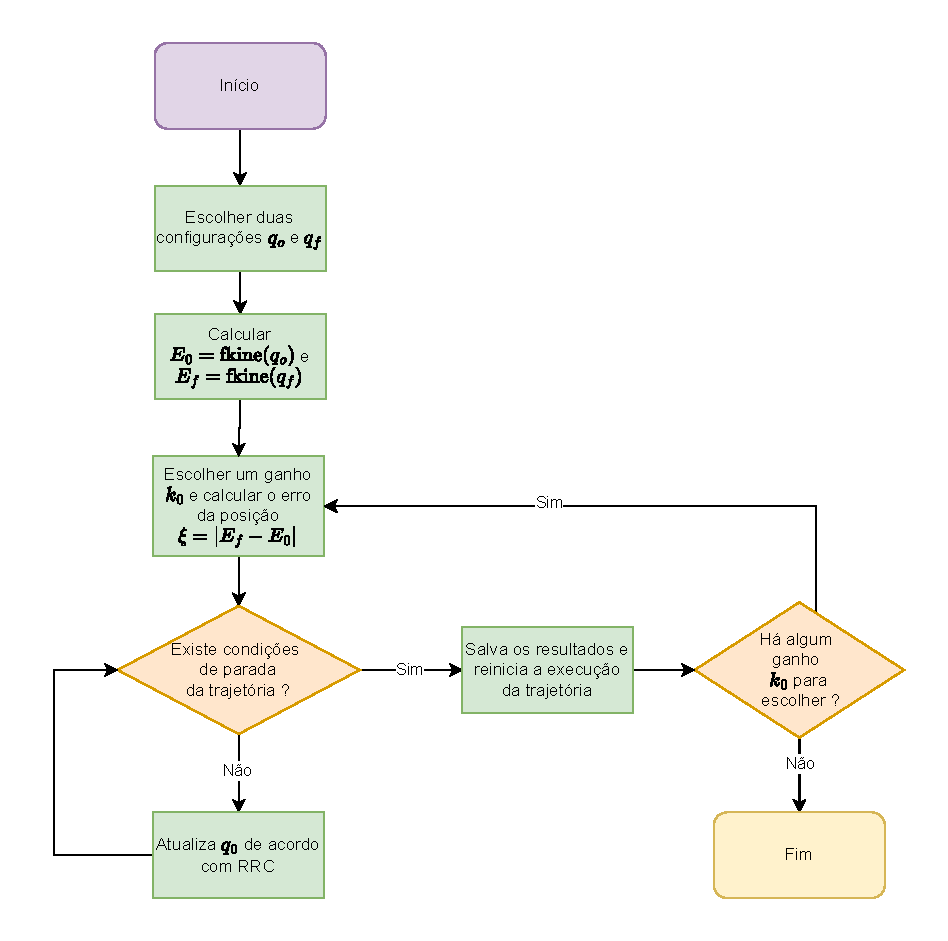
\includegraphics[width=0.8\textwidth]{./Images/exp-flow.pdf}
	\caption{Etapas seguidas na execução de um experimento.}\label{fig:exp-flow}
\end{figure}

Vale ressaltar que devido a natureza complexa da determinação do espaço 
de trabalho do manipulador, procurou-se simplesmente escolher 
os pontos inicias e finais de modo que sejam posições atingíveis, deixando a 
cargo do controlador a execução da melhor trajetória cartesiana entre os dois pontos.
Além disso, a escolha de tais pontos foi feita de maneira aleatória ao longo de diversos experimentos
de modo a não privilegiar nenhuma configuração específica do manipulador.
\cleardoublepage{}
%%% % % % % % % % % % % % % % % % % % % % % % % % % % %
\chapter{Resultados}\label{cap:results}

Este capítulo apresenta os resultados obtidos a partir da simulação da 
execução de trajetórias cartesianas para o manipulador 5R utilizando o esquema 
de controle RRMC. Em cada cenário, foi realizado um conjunto de 4 execuções de 
uma mesma trajetória variando-se o ganho \(k_0\), com o objetivo de avaliar 
a eficácia do controlador em otimizar os índices de desempenho fornecidos, submetido 
a diferentes restrições cinemáticas.

\section{Cenário 1}

No primeiro cenário, a configuração do manipulador muda para trazer algumas posições 
das juntas o mais próximo possível de zero, enquanto a restrição primária imposta pela velocidade 
do efetuador final \(\xi = 0\) mantém a configuração final do manipulador numa solução particular, 
como podemos ver na figura \ref*{fig:exp1-joint-states}. A medida que aumentamos o ganho \(k_0\), a 
configuração do manipulador converge mais rapidamente para a solução final e na figura \ref*{fig:exp1-metric} 
podemos ver os valores menores da distância para os limites mecânicos das juntas sendo obtidos, ao custo 
de um valor de erro ligeiramente maior, como indicado na tabela \ref*{tab:scores-exp1}. Por fim, a figura 
\ref*{fig:exp1-position} mostra a posição do efetuador final constante ao longo de todo o experimento, 
mostrando que a restrição primária não é violada.

\begin{figure}
	\centering
	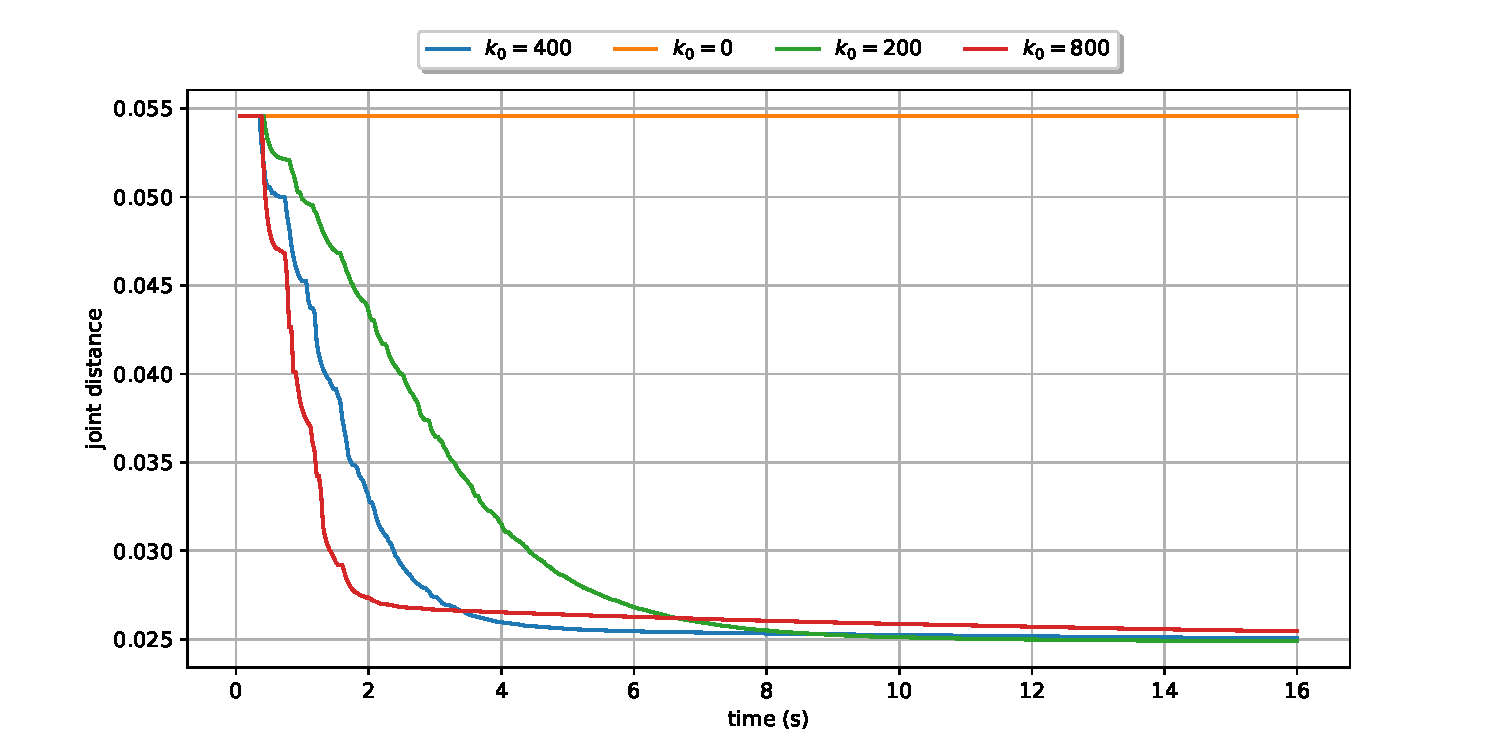
\includegraphics[width=\textwidth]{./Images/2024-06-11-09-23-42/metric_joint_distance.pdf}
	\caption{Diminuição da distância para o limite mecânico das juntas ao longo tempo.}\label{fig:exp1-metric}
\end{figure}

\begin{figure}
	\centering
	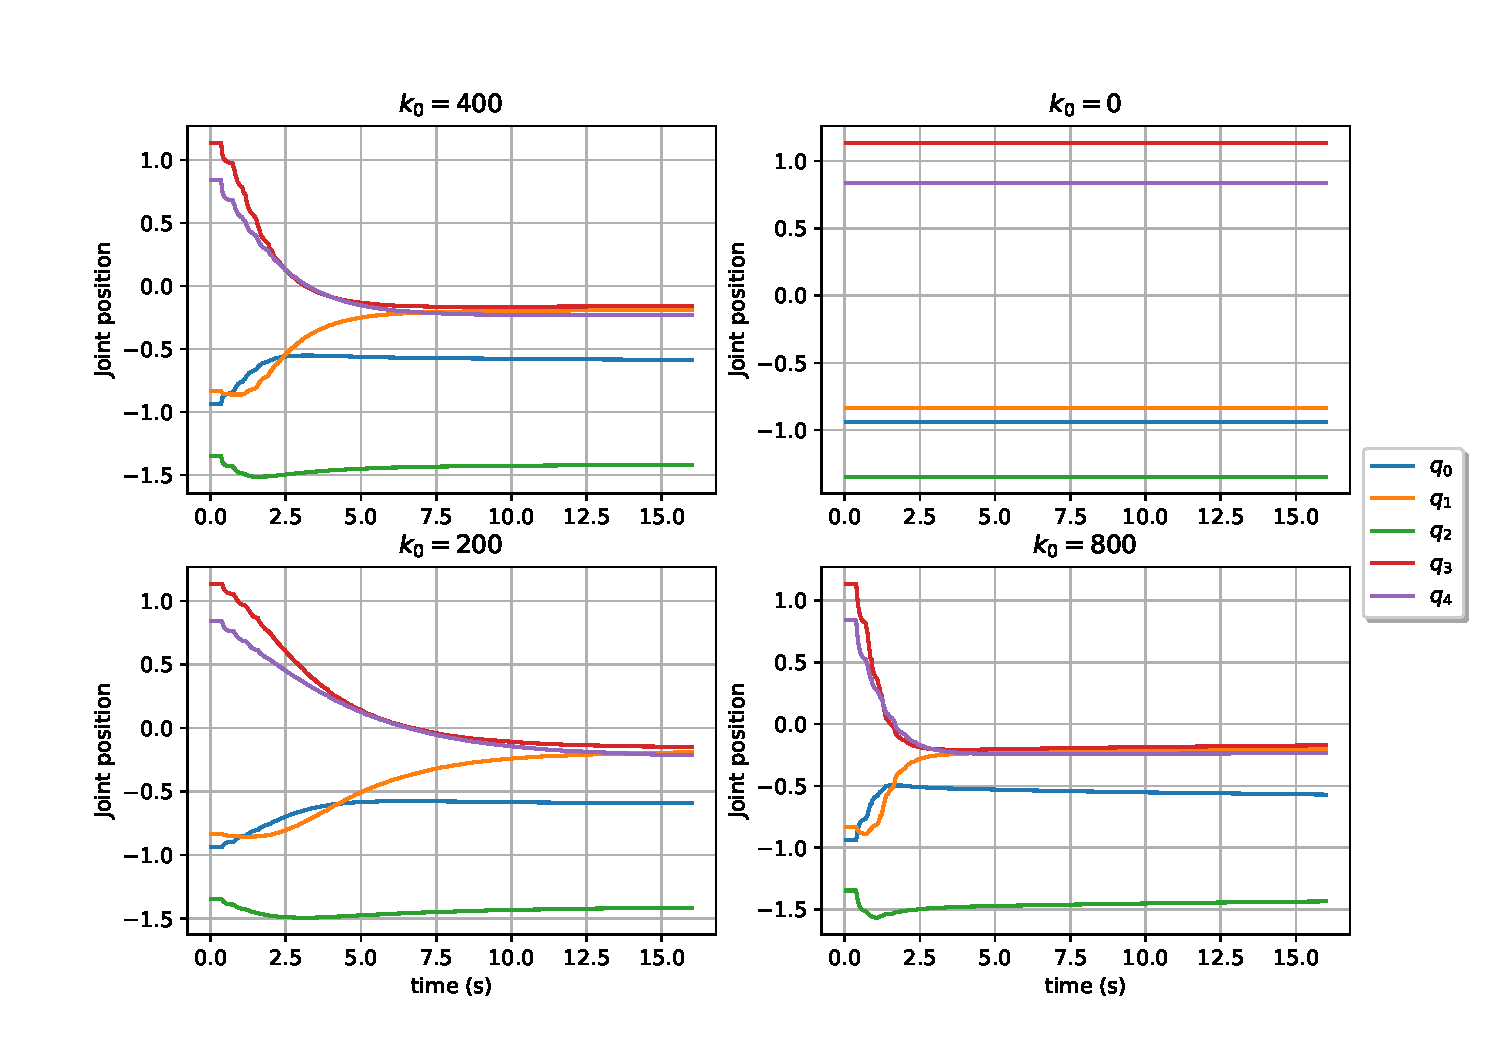
\includegraphics[width=\textwidth]{./Images/2024-06-11-09-23-42/joint_states_joint_distance.pdf}
	\caption{Diferentes valores do ganho, influenciam diretamente na velocidade de convergência para a solução particular.}\label{fig:exp1-joint-states}
\end{figure}

\begin{figure}
	\centering
	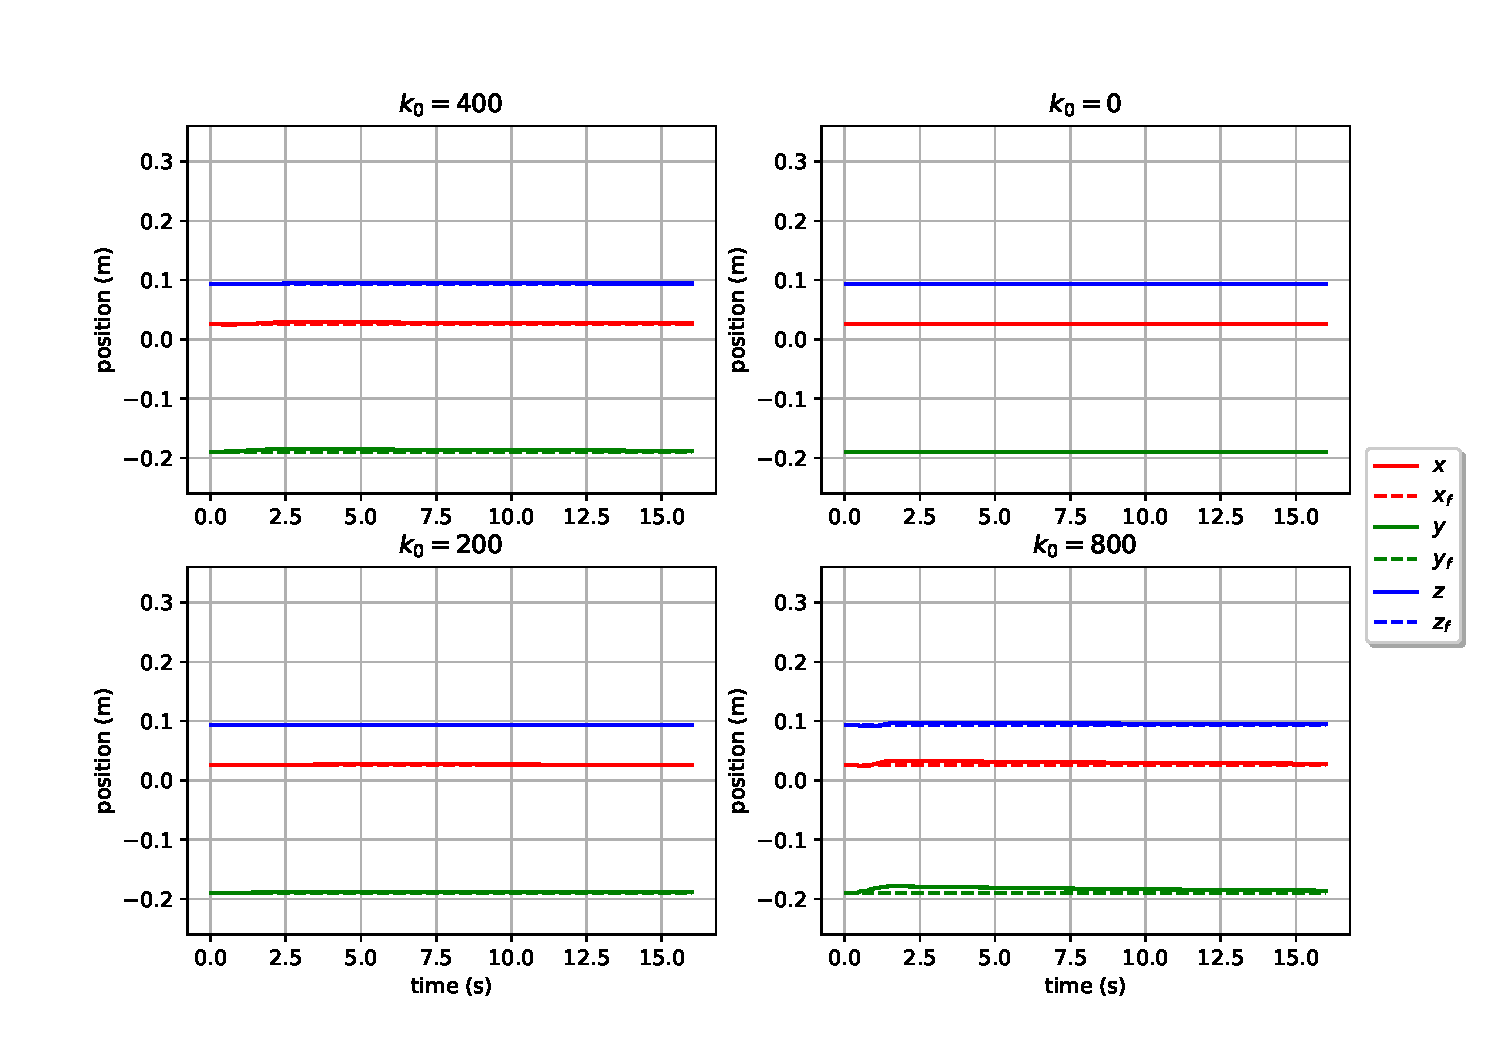
\includegraphics[width=\textwidth]{./Images/2024-06-11-09-23-42/position_joint_distance.pdf}
	\caption{Posição do efetuador final mantém-se constante ao longo do tempo, devido à restrição primária.}\label{fig:exp1-position}
\end{figure}

\begin{table}[htbp]
    \centering
    \begin{tabular}{ccc}
        \toprule
        \( k_0 \) & \( I(w) \)  & Erro posição (m) \\
        \midrule
        0  & \( 0.8729 \) & \( \textbf{1.8535e-06} \) \\
        200  & \( 0.4829 \) & \( 0.0013 \) \\
        400  & \( 0.4488 \) & \( 0.0023 \) \\
        800  & \( \textbf{0.4435} \) & \( 0.0048 \) \\
        \bottomrule
    \end{tabular}
    \caption{Valores de desempenho obtidos na execução dos experimentos do primeiro cenário.}
    \label{tab:scores-exp1}
\end{table}

\section{Cenário 2}
	
No segundo cenário, com a introdução de uma velocidade inicial não nula do efetuador final, isto é \(||\xi|| > 0 \), 
a manipulabilidade muda ao longo da execução da trajetória, aproximando-se de um valor mínimo no seu final (figura \ref*{fig:exp2-metric}). 
A resolução de redundância atualiza a configuração do manipulador de modo manter a manipulabilidade o mais 
alta possível, sem violar a restrição primária.

Observamos novamente que o efeito de introduzir valores crescentes do ganho afeta o erro de posição 
com um pequeno \emph{trade-off} entre a otimização da métrica e a precisão no controle da posição 
do efetuador final (tabelas \ref*{tab:scores-exp2} e \ref*{tab:scores-exp3}), tendo em vista o aumento das 
velocidades das juntas. Esse fenômeno pode ser melhor observado nas figuras \ref*{fig:exp3-joint-states} e 
\ref*{fig:exp3-error}, onde a velocidade das juntas aumenta significativamente ao longo da execução da trajetória, 
e o erro se mantém maior a medida que o ganho \(k_0\) aumenta. Isso pode ser explicado pelo fato 
de que a métrica de desempenho, nesse caso a distância das juntas (figura \ref*{fig:exp3-metric}), é otimizada como um objetivo secundário 
à restrição imposta por \(\xi\), e a escolha de trajetórias onde os valores da métricas estão muito distantes
 do valor ótimo, acabam tornando o processo de otimização mais difícil, necessitando assim um valor de \(k_0\) 
 maior para convergir para a solução ótima.

\begin{figure}
	\centering
	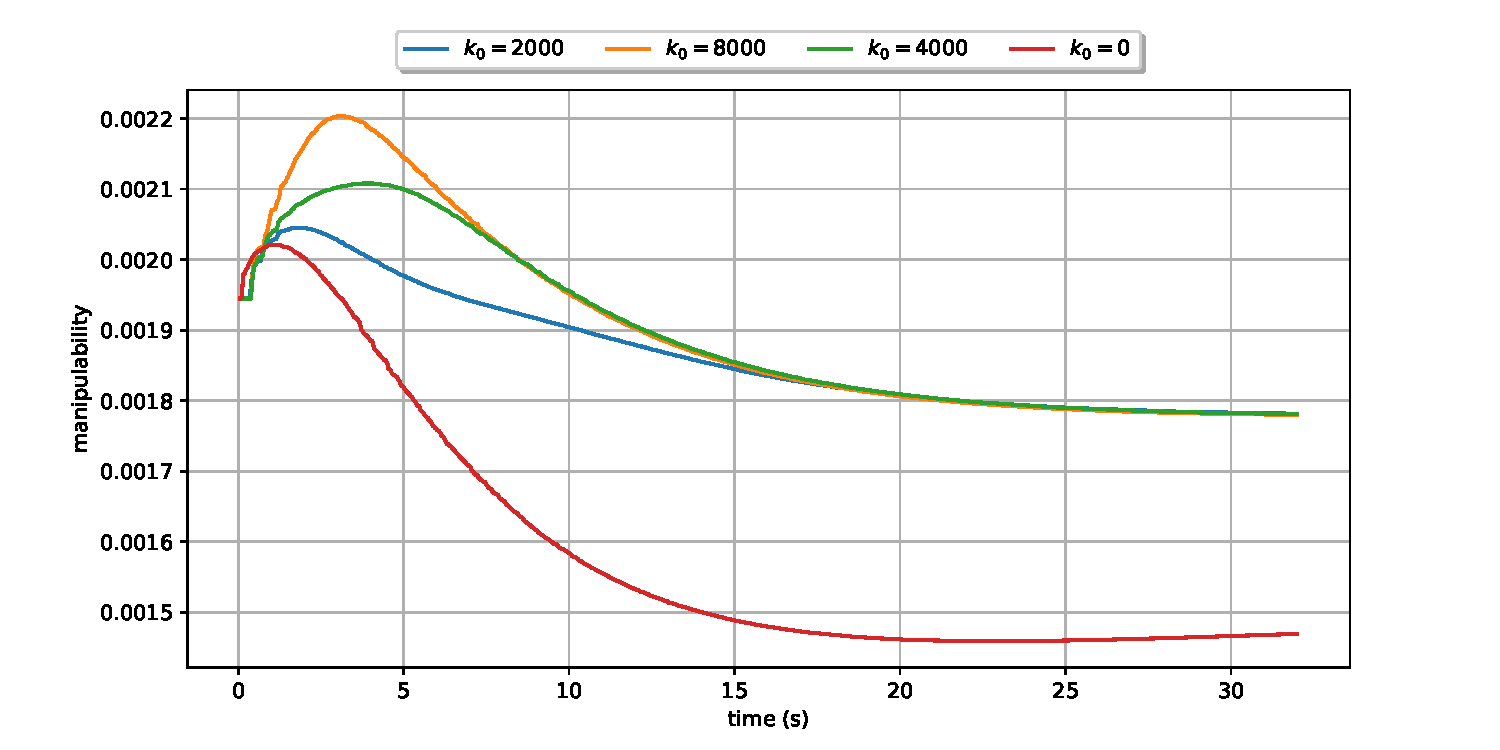
\includegraphics[width=\textwidth]{./Images/2024-06-11-09-17-48/metric_manipulability.pdf}
	\caption{Manipulabilidade em função do tempo para cada trajetória executada no segundo cenário.}\label{fig:exp2-metric}
\end{figure}

\begin{table}[htbp]
    \centering
    \begin{tabular}{ccc}
        \toprule
        \( k_0 \) & \( I(w) \)  & Erro posição (m) \\
        \midrule
        0  & \( 0.0507 \) & \( \textbf{0.0138} \) \\
        2000  & \( 0.0597 \) & \( 0.0150 \) \\
        4000  & \( 0.0606 \) & \( 0.0151 \) \\
        8000  & \( \textbf{0.0609} \) & \( 0.0149 \) \\
        \bottomrule
    \end{tabular}
    \caption{Valores de desempenho obtidos na execução dos experimentos do segundo cenário.}
    \label{tab:scores-exp2}
\end{table}

\begin{figure}
	\centering
	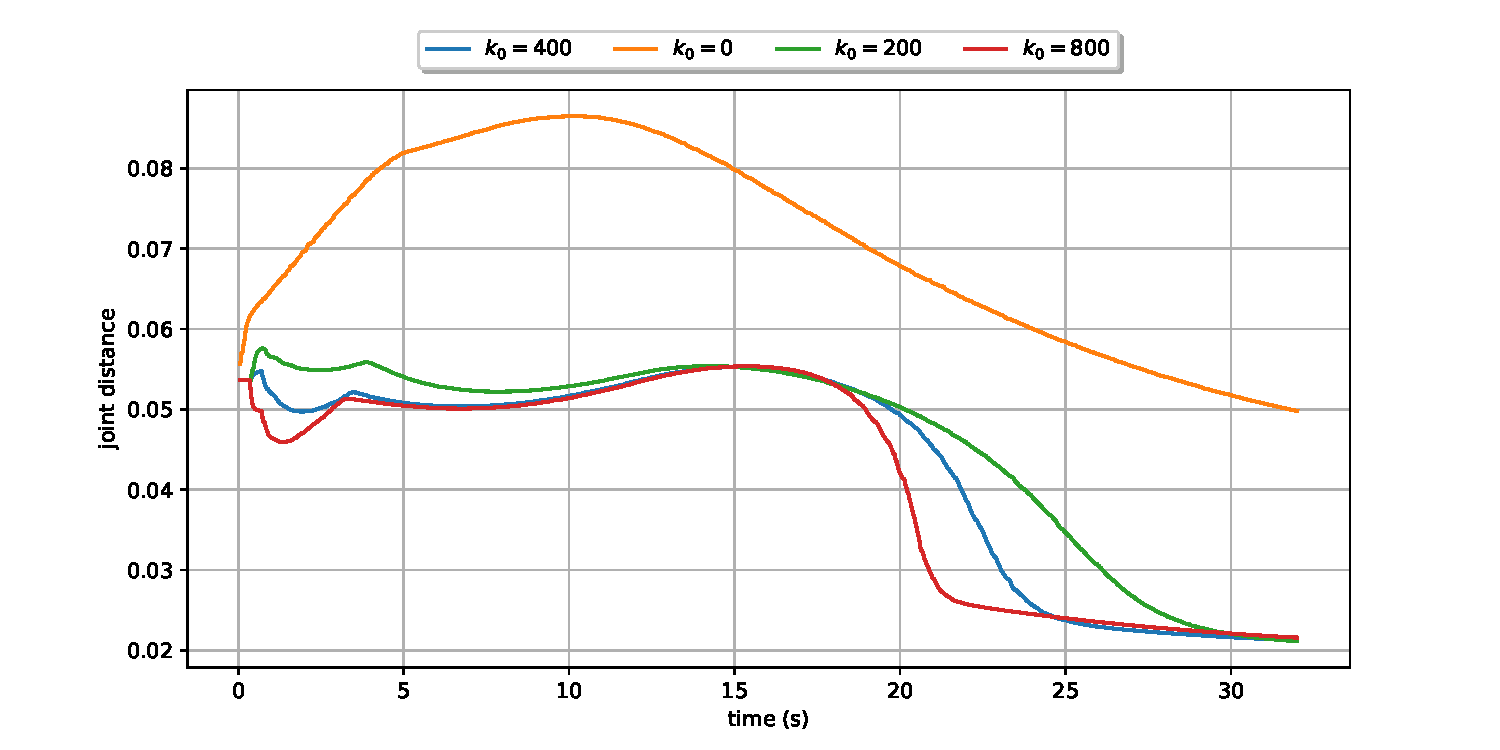
\includegraphics[width=\textwidth]{./Images/2024-07-02-14-04-38/metric_joint_distance.pdf}
	\caption{Otimizando distância das juntas no segundo cenário.}\label{fig:exp3-metric}
\end{figure}

\begin{figure}
	\centering
	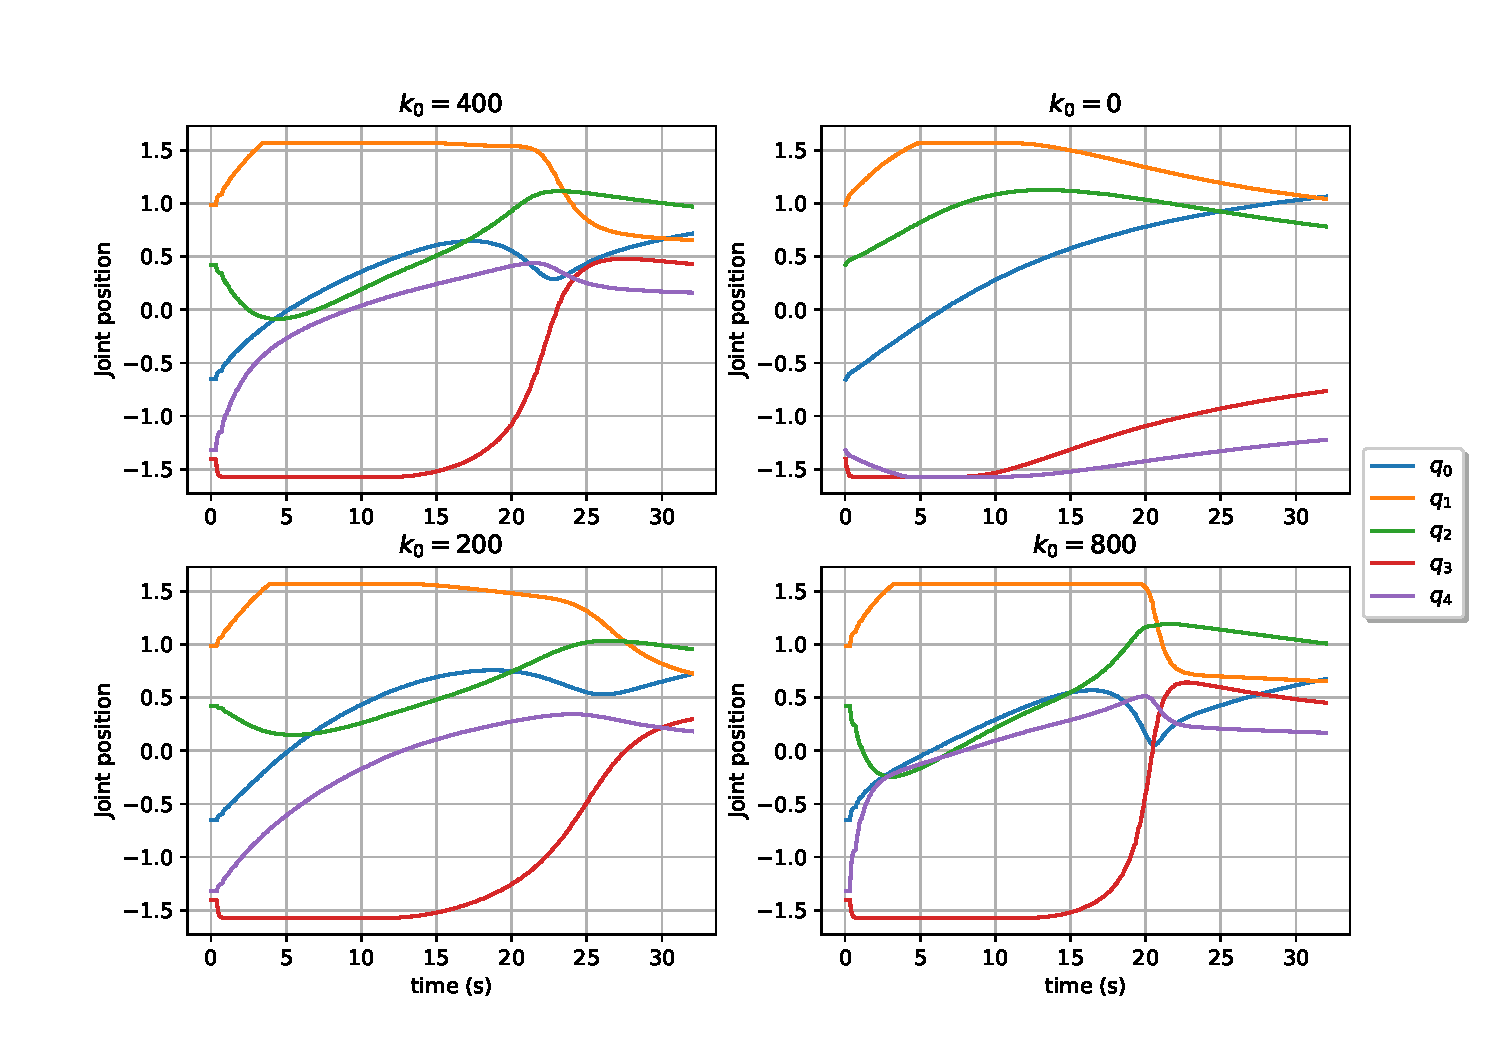
\includegraphics[width=\textwidth]{./Images/2024-07-02-14-04-38/joint_states_joint_distance.pdf}
	\caption{Em determinadas trajetórias, o impacto do ganho na velocidade das juntas é significativo.}\label{fig:exp3-joint-states}
\end{figure}

\begin{figure}
	\centering
	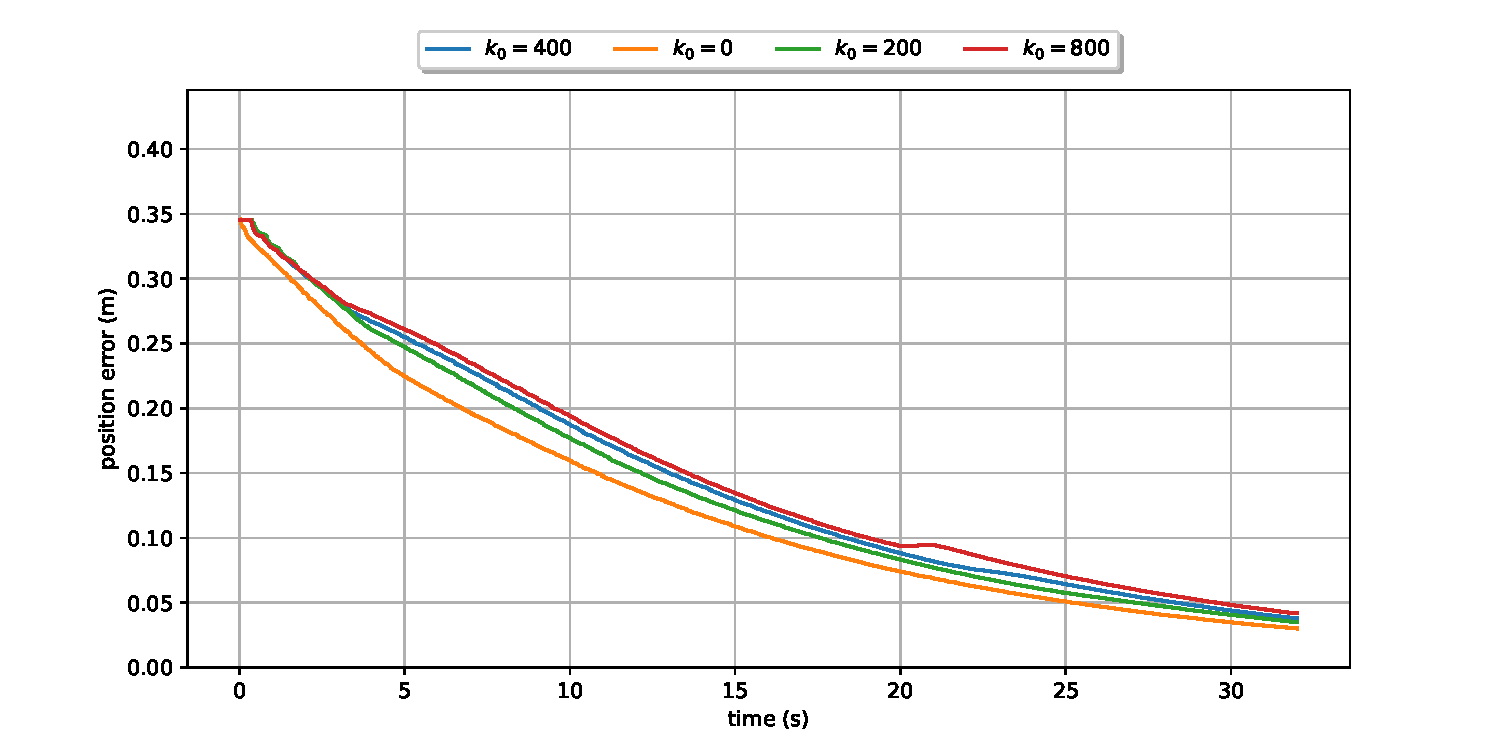
\includegraphics[width=\textwidth]{./Images/2024-07-02-14-04-38/position_error_joint_distance.pdf}
	\caption{Erro da posição ao longo do tempo para o segundo cenário.}\label{fig:exp3-error}
\end{figure}

\begin{table}[htbp]
    \centering
    \begin{tabular}{ccc}
        \toprule
        \( k_0 \) & \( I(w) \) & Erro posição (m) \\
        \midrule
        0  & \( 2.2622 \) & \( \textbf{0.0301} \) \\
        200  & \( 1.4727 \) & \( 0.0350 \) \\
        400  & \( 1.3777 \) & \( 0.0379 \) \\
        800  & \( \textbf{1.3251} \) & \( 0.0418 \) \\
        \bottomrule
    \end{tabular}
    \caption{Valores de desempenho (métrica distância das juntas) obtidos na execução dos experimentos no segundo cenário.}
    \label{tab:scores-exp3}
\end{table}

\cleardoublepage{}
%%% % % % % % % % % % % % % % % % % % % % % % % % % % %
\chapter{Conclusão}\label{cap:conclusao}

Este trabalho discutiu a aplicação de esquemas de controle com resolução de 
redundância para abordar os desafios impostos pelas singularidades na cinemática 
diferencial inversa de um manipulador serial com cinco graus de liberdade. Foi proposto ambiente completamente
simulado para testar e validar a estratégia de controle, proporcionando também uma comunicação robusta 
entre controlador e o modelo virtual do manipulador usando o Sistema Operacional de Robôs (ROS). 
A abordagem foi avaliada em cenários distintos, propiciando uma análise qualitativa da execução de
trajetórias em diferentes condições de restrições cinemáticas e de desempenho do manipulador.

Perspectivas futuras para o trabalho, incluem o estudo da escolha ótima de um ganho \(k_0\), visando otimizar 
o desempenho do manipulador em diferentes cenários e também uma análise teórica/estatística mais aprofundada dos resultados obtidos, com o objetivo de avaliar a robustez do
controlador e a convergência para soluções ótimas. Além disso, é desejável explorar cadeias cinemáticas 
mais complexas, como as dos manipuladores do tipo \emph{elbow} e \emph{wrist}, que possuem um maior 
grau de redundância tipicamente maior que 7, permitindo a resolução não so a nível do controle da posição, mas 
também da orientação do efetuador final. Vale ressaltar também que uma continuidade natural para o trabalho 
é a transferência dos resultados para um robô real e a integração em um \emph{framework} de planejamento de trajetórias, permitindo
a validação do esquema de controle em cenários mais realistas e desafiadores.
\cleardoublepage{}
%%% % % % % % % % % % % % % % % % % % % % % % % % % % %
%%% % % % % % % % % % % % % % % % % % % % % % % % % % %
\markright{Bibliografia}
\renewcommand\bibname{Bibliografia}

% % % % % % % % % % % % % % % % % % % % % % % % % % %
% Definir estilo bibliográfico  % % % % % % % % % % %
% % % % % % % % % % % % % % % % % % % % % % % % % % %
%\bibliographystyle{alpha}
\bibliographystyle{apalike}
%\bibliographystyle{ieeetr}
%%
{
	\addcontentsline{toc}{chapter}{Bibliografia}
	\bibliography{Ref/SampleReferences}
}
\cleardoublepage{}
%%% % % % % % % % % % % % % % % % % % % % % % % % % % %
%%% % % % % % % % % % % % % % % % % % % % % % % % % % %
\end{document}
